\documentclass[twoside]{book}

% Packages required by doxygen
\usepackage{fixltx2e}
\usepackage{calc}
\usepackage{doxygen}
\usepackage[export]{adjustbox} % also loads graphicx
\usepackage{graphicx}
\usepackage[utf8]{inputenc}
\usepackage{makeidx}
\usepackage{multicol}
\usepackage{multirow}
\PassOptionsToPackage{warn}{textcomp}
\usepackage{textcomp}
\usepackage[nointegrals]{wasysym}
\usepackage[table]{xcolor}

% Font selection
\usepackage[T1]{fontenc}
\usepackage[scaled=.90]{helvet}
\usepackage{courier}
\usepackage{amssymb}
\usepackage{sectsty}
\renewcommand{\familydefault}{\sfdefault}
\allsectionsfont{%
  \fontseries{bc}\selectfont%
  \color{darkgray}%
}
\renewcommand{\DoxyLabelFont}{%
  \fontseries{bc}\selectfont%
  \color{darkgray}%
}
\newcommand{\+}{\discretionary{\mbox{\scriptsize$\hookleftarrow$}}{}{}}

% Page & text layout
\usepackage{geometry}
\geometry{%
  a4paper,%
  top=2.5cm,%
  bottom=2.5cm,%
  left=2.5cm,%
  right=2.5cm%
}
\tolerance=750
\hfuzz=15pt
\hbadness=750
\setlength{\emergencystretch}{15pt}
\setlength{\parindent}{0cm}
\setlength{\parskip}{3ex plus 2ex minus 2ex}
\makeatletter
\renewcommand{\paragraph}{%
  \@startsection{paragraph}{4}{0ex}{-1.0ex}{1.0ex}{%
    \normalfont\normalsize\bfseries\SS@parafont%
  }%
}
\renewcommand{\subparagraph}{%
  \@startsection{subparagraph}{5}{0ex}{-1.0ex}{1.0ex}{%
    \normalfont\normalsize\bfseries\SS@subparafont%
  }%
}
\makeatother

% Headers & footers
\usepackage{fancyhdr}
\pagestyle{fancyplain}
\fancyhead[LE]{\fancyplain{}{\bfseries\thepage}}
\fancyhead[CE]{\fancyplain{}{}}
\fancyhead[RE]{\fancyplain{}{\bfseries\leftmark}}
\fancyhead[LO]{\fancyplain{}{\bfseries\rightmark}}
\fancyhead[CO]{\fancyplain{}{}}
\fancyhead[RO]{\fancyplain{}{\bfseries\thepage}}
\fancyfoot[LE]{\fancyplain{}{}}
\fancyfoot[CE]{\fancyplain{}{}}
\fancyfoot[RE]{\fancyplain{}{\bfseries\scriptsize Generated by Doxygen }}
\fancyfoot[LO]{\fancyplain{}{\bfseries\scriptsize Generated by Doxygen }}
\fancyfoot[CO]{\fancyplain{}{}}
\fancyfoot[RO]{\fancyplain{}{}}
\renewcommand{\footrulewidth}{0.4pt}
\renewcommand{\chaptermark}[1]{%
  \markboth{#1}{}%
}
\renewcommand{\sectionmark}[1]{%
  \markright{\thesection\ #1}%
}

% Indices & bibliography
\usepackage{natbib}
\usepackage[titles]{tocloft}
\setcounter{tocdepth}{3}
\setcounter{secnumdepth}{5}
\makeindex

% Hyperlinks (required, but should be loaded last)
\usepackage{ifpdf}
\ifpdf
  \usepackage[pdftex,pagebackref=true]{hyperref}
\else
  \usepackage[ps2pdf,pagebackref=true]{hyperref}
\fi
\hypersetup{%
  colorlinks=true,%
  linkcolor=blue,%
  citecolor=blue,%
  unicode%
}

% Custom commands
\newcommand{\clearemptydoublepage}{%
  \newpage{\pagestyle{empty}\cleardoublepage}%
}

\usepackage{caption}
\captionsetup{labelsep=space,justification=centering,font={bf},singlelinecheck=off,skip=4pt,position=top}

%===== C O N T E N T S =====

\begin{document}

% Titlepage & ToC
\hypersetup{pageanchor=false,
             bookmarksnumbered=true,
             pdfencoding=unicode
            }
\pagenumbering{alph}
\begin{titlepage}
\vspace*{7cm}
\begin{center}%
{\Large My Project }\\
\vspace*{1cm}
{\large Generated by Doxygen 1.8.14}\\
\end{center}
\end{titlepage}
\clearemptydoublepage
\pagenumbering{roman}
\tableofcontents
\clearemptydoublepage
\pagenumbering{arabic}
\hypersetup{pageanchor=true}

%--- Begin generated contents ---
\chapter{Hierarchical Index}
\section{Class Hierarchy}
This inheritance list is sorted roughly, but not completely, alphabetically\+:\begin{DoxyCompactList}
\item \contentsline{section}{game.\+Board}{\pageref{classgame_1_1_board}}{}
\item \contentsline{section}{game.\+Game}{\pageref{classgame_1_1_game}}{}
\item \contentsline{section}{G\+U\+I.\+Game\+G\+UI}{\pageref{class_g_u_i_1_1_game_g_u_i}}{}
\item J\+Button\begin{DoxyCompactList}
\item \contentsline{section}{G\+U\+I.\+Button}{\pageref{class_g_u_i_1_1_button}}{}
\end{DoxyCompactList}
\item J\+Panel\begin{DoxyCompactList}
\item \contentsline{section}{G\+U\+I.\+Board\+G\+UI}{\pageref{class_g_u_i_1_1_board_g_u_i}}{}
\end{DoxyCompactList}
\item \contentsline{section}{pieces.\+Pieces}{\pageref{classpieces_1_1_pieces}}{}
\begin{DoxyCompactList}
\item \contentsline{section}{pieces.\+Bishop}{\pageref{classpieces_1_1_bishop}}{}
\item \contentsline{section}{pieces.\+Hopper}{\pageref{classpieces_1_1_hopper}}{}
\item \contentsline{section}{pieces.\+King}{\pageref{classpieces_1_1_king}}{}
\item \contentsline{section}{pieces.\+Knight}{\pageref{classpieces_1_1_knight}}{}
\item \contentsline{section}{pieces.\+Pawn}{\pageref{classpieces_1_1_pawn}}{}
\item \contentsline{section}{pieces.\+Queen}{\pageref{classpieces_1_1_queen}}{}
\item \contentsline{section}{pieces.\+Rook}{\pageref{classpieces_1_1_rook}}{}
\item \contentsline{section}{pieces.\+Wizard}{\pageref{classpieces_1_1_wizard}}{}
\end{DoxyCompactList}
\item \contentsline{section}{game.\+Player}{\pageref{classgame_1_1_player}}{}
\item \contentsline{section}{pieces.\+Type}{\pageref{enumpieces_1_1_type}}{}
\end{DoxyCompactList}

\chapter{Class Index}
\section{Class List}
Here are the classes, structs, unions and interfaces with brief descriptions\+:\begin{DoxyCompactList}
\item\contentsline{section}{\mbox{\hyperlink{classpieces_1_1_bishop}{pieces.\+Bishop}} }{\pageref{classpieces_1_1_bishop}}{}
\item\contentsline{section}{\mbox{\hyperlink{classgame_1_1_board}{game.\+Board}} }{\pageref{classgame_1_1_board}}{}
\item\contentsline{section}{\mbox{\hyperlink{class_g_u_i_1_1_board_g_u_i}{G\+U\+I.\+Board\+G\+UI}} }{\pageref{class_g_u_i_1_1_board_g_u_i}}{}
\item\contentsline{section}{\mbox{\hyperlink{class_g_u_i_1_1_button}{G\+U\+I.\+Button}} }{\pageref{class_g_u_i_1_1_button}}{}
\item\contentsline{section}{\mbox{\hyperlink{classgame_1_1_game}{game.\+Game}} }{\pageref{classgame_1_1_game}}{}
\item\contentsline{section}{\mbox{\hyperlink{class_g_u_i_1_1_game_g_u_i}{G\+U\+I.\+Game\+G\+UI}} }{\pageref{class_g_u_i_1_1_game_g_u_i}}{}
\item\contentsline{section}{\mbox{\hyperlink{classpieces_1_1_hopper}{pieces.\+Hopper}} }{\pageref{classpieces_1_1_hopper}}{}
\item\contentsline{section}{\mbox{\hyperlink{classpieces_1_1_king}{pieces.\+King}} }{\pageref{classpieces_1_1_king}}{}
\item\contentsline{section}{\mbox{\hyperlink{classpieces_1_1_knight}{pieces.\+Knight}} }{\pageref{classpieces_1_1_knight}}{}
\item\contentsline{section}{\mbox{\hyperlink{classpieces_1_1_pawn}{pieces.\+Pawn}} }{\pageref{classpieces_1_1_pawn}}{}
\item\contentsline{section}{\mbox{\hyperlink{classpieces_1_1_pieces}{pieces.\+Pieces}} }{\pageref{classpieces_1_1_pieces}}{}
\item\contentsline{section}{\mbox{\hyperlink{classgame_1_1_player}{game.\+Player}} }{\pageref{classgame_1_1_player}}{}
\item\contentsline{section}{\mbox{\hyperlink{classpieces_1_1_queen}{pieces.\+Queen}} }{\pageref{classpieces_1_1_queen}}{}
\item\contentsline{section}{\mbox{\hyperlink{classpieces_1_1_rook}{pieces.\+Rook}} }{\pageref{classpieces_1_1_rook}}{}
\item\contentsline{section}{\mbox{\hyperlink{enumpieces_1_1_type}{pieces.\+Type}} }{\pageref{enumpieces_1_1_type}}{}
\item\contentsline{section}{\mbox{\hyperlink{classpieces_1_1_wizard}{pieces.\+Wizard}} }{\pageref{classpieces_1_1_wizard}}{}
\end{DoxyCompactList}

\chapter{Class Documentation}
\hypertarget{classpieces_1_1_bishop}{}\section{pieces.\+Bishop Class Reference}
\label{classpieces_1_1_bishop}\index{pieces.\+Bishop@{pieces.\+Bishop}}
Inheritance diagram for pieces.\+Bishop\+:\begin{figure}[H]
\begin{center}
\leavevmode
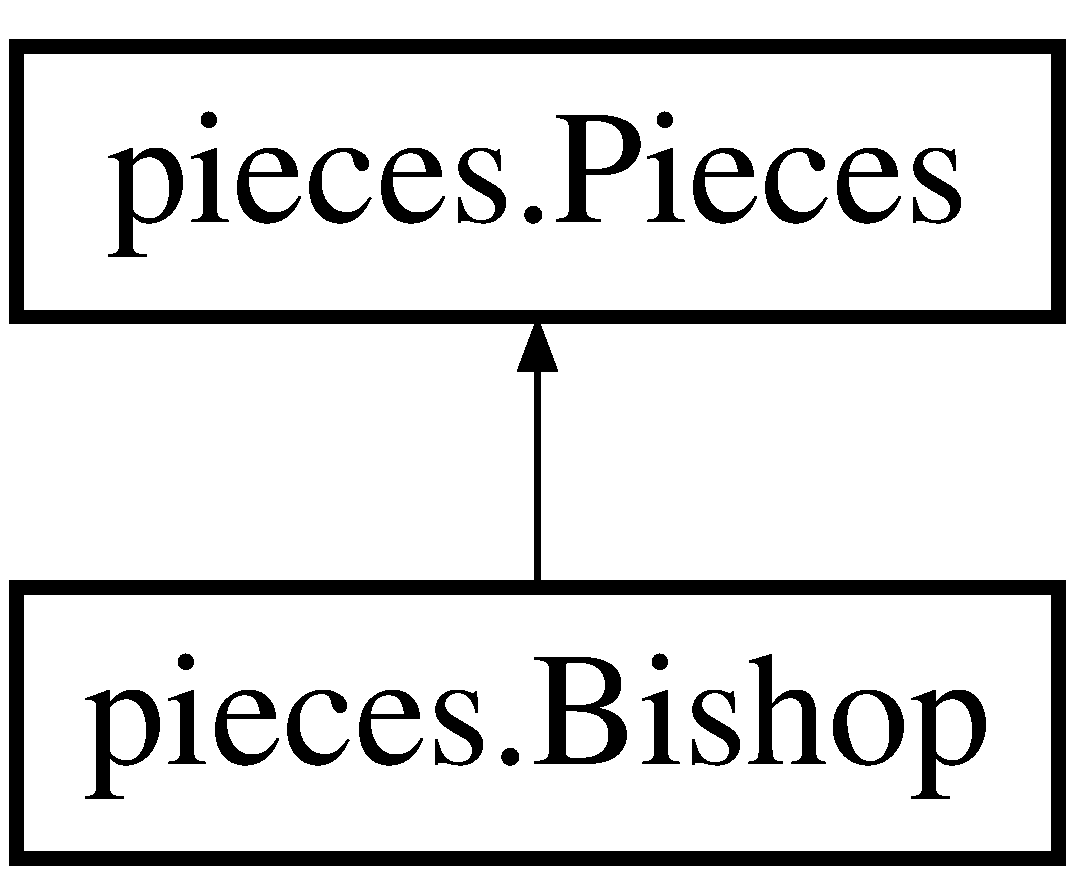
\includegraphics[height=2.000000cm]{classpieces_1_1_bishop}
\end{center}
\end{figure}
\subsection*{Public Member Functions}
\begin{DoxyCompactItemize}
\item 
\mbox{\hyperlink{classpieces_1_1_bishop_ac957b1b3befde750ebd7b8789a4e597f}{Bishop}} (int \mbox{\hyperlink{classpieces_1_1_pieces_ac5178f9b8a6b0c4235851475081249f3}{x}}, int \mbox{\hyperlink{classpieces_1_1_pieces_a66d911734967a8ced1b9792fe900fadb}{y}}, \mbox{\hyperlink{classgame_1_1_player}{Player}} \mbox{\hyperlink{classpieces_1_1_pieces_a49f35044dd36e5c4b04261a8ea54ad0c}{player}})
\item 
boolean \mbox{\hyperlink{classpieces_1_1_bishop_a183c86371bda01aa8567b245a4977dab}{is\+Valid\+Move}} (int newX, int newY)
\item 
List$<$ int\mbox{[}$\,$\mbox{]}$>$ \mbox{\hyperlink{classpieces_1_1_bishop_a3bdcfb9a3b44569aee1d5d4e5aa7333d}{moving}} (int newX, int newY)
\end{DoxyCompactItemize}
\subsection*{Additional Inherited Members}


\subsection{Detailed Description}
\mbox{\hyperlink{classpieces_1_1_bishop}{Bishop}} class 

The bishop can move any number of squares diagonally, but may not leap over other pieces. 

\subsection{Constructor \& Destructor Documentation}
\mbox{\Hypertarget{classpieces_1_1_bishop_ac957b1b3befde750ebd7b8789a4e597f}\label{classpieces_1_1_bishop_ac957b1b3befde750ebd7b8789a4e597f}} 
\index{pieces\+::\+Bishop@{pieces\+::\+Bishop}!Bishop@{Bishop}}
\index{Bishop@{Bishop}!pieces\+::\+Bishop@{pieces\+::\+Bishop}}
\subsubsection{\texorpdfstring{Bishop()}{Bishop()}}
{\footnotesize\ttfamily pieces.\+Bishop.\+Bishop (\begin{DoxyParamCaption}\item[{int}]{x,  }\item[{int}]{y,  }\item[{\mbox{\hyperlink{classgame_1_1_player}{Player}}}]{player }\end{DoxyParamCaption})\hspace{0.3cm}{\ttfamily [inline]}}

initialize bishop attributes 
\begin{DoxyParams}{Parameters}
{\em x} & the initial rank position \\
\hline
{\em y} & the initial file position \\
\hline
{\em player} & the player piece belong to \\
\hline
\end{DoxyParams}


\subsection{Member Function Documentation}
\mbox{\Hypertarget{classpieces_1_1_bishop_a183c86371bda01aa8567b245a4977dab}\label{classpieces_1_1_bishop_a183c86371bda01aa8567b245a4977dab}} 
\index{pieces\+::\+Bishop@{pieces\+::\+Bishop}!is\+Valid\+Move@{is\+Valid\+Move}}
\index{is\+Valid\+Move@{is\+Valid\+Move}!pieces\+::\+Bishop@{pieces\+::\+Bishop}}
\subsubsection{\texorpdfstring{is\+Valid\+Move()}{isValidMove()}}
{\footnotesize\ttfamily boolean pieces.\+Bishop.\+is\+Valid\+Move (\begin{DoxyParamCaption}\item[{int}]{newX,  }\item[{int}]{newY }\end{DoxyParamCaption})\hspace{0.3cm}{\ttfamily [inline]}}

check whether bishop is moved by its own rule; bishop could only move diagonally 
\begin{DoxyParams}{Parameters}
{\em newX} & destination rank of the piece \\
\hline
{\em newY} & destination file of the piece \\
\hline
\end{DoxyParams}
\begin{DoxyReturn}{Returns}
whether this step is a valid move 
\end{DoxyReturn}
\mbox{\Hypertarget{classpieces_1_1_bishop_a3bdcfb9a3b44569aee1d5d4e5aa7333d}\label{classpieces_1_1_bishop_a3bdcfb9a3b44569aee1d5d4e5aa7333d}} 
\index{pieces\+::\+Bishop@{pieces\+::\+Bishop}!moving@{moving}}
\index{moving@{moving}!pieces\+::\+Bishop@{pieces\+::\+Bishop}}
\subsubsection{\texorpdfstring{moving()}{moving()}}
{\footnotesize\ttfamily List$<$int\mbox{[}$\,$\mbox{]}$>$ pieces.\+Bishop.\+moving (\begin{DoxyParamCaption}\item[{int}]{newX,  }\item[{int}]{newY }\end{DoxyParamCaption})\hspace{0.3cm}{\ttfamily [inline]}}

store the passing positions a helper function for later check leap over other pieces 
\begin{DoxyParams}{Parameters}
{\em newX} & destination rank of the piece \\
\hline
{\em newY} & destination file of the piece \\
\hline
\end{DoxyParams}
\begin{DoxyReturn}{Returns}
a list of squares that the piece passing 
\end{DoxyReturn}


The documentation for this class was generated from the following file\+:\begin{DoxyCompactItemize}
\item 
src/pieces/Bishop.\+java\end{DoxyCompactItemize}

\hypertarget{classgame_1_1_board}{}\section{game.\+Board Class Reference}
\label{classgame_1_1_board}\index{game.\+Board@{game.\+Board}}
\subsection*{Public Member Functions}
\begin{DoxyCompactItemize}
\item 
\mbox{\hyperlink{classgame_1_1_board_afd26ab4fbb8f5ce04a9bf8a69782c4db}{Board}} (int rank, int file, \mbox{\hyperlink{classgame_1_1_player}{Player}} player0, \mbox{\hyperlink{classgame_1_1_player}{Player}} player1)
\item 
void \mbox{\hyperlink{classgame_1_1_board_a9955ee857e479d54216ce6d6a12e8145}{set\+Pieces}} ()
\item 
boolean \mbox{\hyperlink{classgame_1_1_board_af34ca67982d198cf4acdaa8baa12c96b}{check\+Valid}} (\mbox{\hyperlink{classgame_1_1_player}{Player}} player, int prevX, int prevY, int newX, int newY)
\item 
\mbox{\hyperlink{classpieces_1_1_pieces}{Pieces}} \mbox{\hyperlink{classgame_1_1_board_a512879cf8a8705450f5e94ecb147b1ff}{put\+Pieces}} (\mbox{\hyperlink{classgame_1_1_player}{Player}} player, int prevX, int prevY, int newX, int newY)
\item 
boolean \mbox{\hyperlink{classgame_1_1_board_a631a4ad5cde58f7263ffc57b97458faf}{in\+Check}} (\mbox{\hyperlink{classgame_1_1_player}{Player}} moving\+Player, \mbox{\hyperlink{classgame_1_1_player}{Player}} opponent)
\item 
boolean \mbox{\hyperlink{classgame_1_1_board_a95871969333ec29f0299b1bbeb277121}{is\+Checkmate}} (\mbox{\hyperlink{classgame_1_1_player}{Player}} moving\+Player, \mbox{\hyperlink{classgame_1_1_player}{Player}} opponent)
\item 
boolean \mbox{\hyperlink{classgame_1_1_board_a7f5f2366e087babfd08a82afc332771c}{is\+Stalemate}} (\mbox{\hyperlink{classgame_1_1_player}{Player}} moving\+Player, \mbox{\hyperlink{classgame_1_1_player}{Player}} opponent)
\end{DoxyCompactItemize}
\subsection*{Public Attributes}
\begin{DoxyCompactItemize}
\item 
\mbox{\hyperlink{classpieces_1_1_pieces}{Pieces}} \mbox{[}$\,$\mbox{]}\mbox{[}$\,$\mbox{]} \mbox{\hyperlink{classgame_1_1_board_a88a0b3ed05aed6166209784f05fd218d}{board}}
\end{DoxyCompactItemize}


\subsection{Detailed Description}
\mbox{\hyperlink{classgame_1_1_board}{Board}} Class contains game logic, piece move validation check and game end condition check 

\subsection{Constructor \& Destructor Documentation}
\mbox{\Hypertarget{classgame_1_1_board_afd26ab4fbb8f5ce04a9bf8a69782c4db}\label{classgame_1_1_board_afd26ab4fbb8f5ce04a9bf8a69782c4db}} 
\index{game\+::\+Board@{game\+::\+Board}!Board@{Board}}
\index{Board@{Board}!game\+::\+Board@{game\+::\+Board}}
\subsubsection{\texorpdfstring{Board()}{Board()}}
{\footnotesize\ttfamily game.\+Board.\+Board (\begin{DoxyParamCaption}\item[{int}]{rank,  }\item[{int}]{file,  }\item[{\mbox{\hyperlink{classgame_1_1_player}{Player}}}]{player0,  }\item[{\mbox{\hyperlink{classgame_1_1_player}{Player}}}]{player1 }\end{DoxyParamCaption})\hspace{0.3cm}{\ttfamily [inline]}}

initialize board attributes 
\begin{DoxyParams}{Parameters}
{\em rank} & the number of ranks \\
\hline
{\em file} & the number of files \\
\hline
{\em player0} & the upper player \\
\hline
{\em player1} & the downwards player \\
\hline
\end{DoxyParams}


\subsection{Member Function Documentation}
\mbox{\Hypertarget{classgame_1_1_board_af34ca67982d198cf4acdaa8baa12c96b}\label{classgame_1_1_board_af34ca67982d198cf4acdaa8baa12c96b}} 
\index{game\+::\+Board@{game\+::\+Board}!check\+Valid@{check\+Valid}}
\index{check\+Valid@{check\+Valid}!game\+::\+Board@{game\+::\+Board}}
\subsubsection{\texorpdfstring{check\+Valid()}{checkValid()}}
{\footnotesize\ttfamily boolean game.\+Board.\+check\+Valid (\begin{DoxyParamCaption}\item[{\mbox{\hyperlink{classgame_1_1_player}{Player}}}]{player,  }\item[{int}]{prevX,  }\item[{int}]{prevY,  }\item[{int}]{newX,  }\item[{int}]{newY }\end{DoxyParamCaption})\hspace{0.3cm}{\ttfamily [inline]}}

check whether this step is valid; 
\begin{DoxyParams}{Parameters}
{\em player} & the player who is moving pieces \\
\hline
{\em prevX} & the start rank position \\
\hline
{\em prevY} & the start file position \\
\hline
{\em newX} & the destination of rank position \\
\hline
{\em newY} & the destination of file position \\
\hline
\end{DoxyParams}
\begin{DoxyReturn}{Returns}
whether this step is valid 
\end{DoxyReturn}
\mbox{\Hypertarget{classgame_1_1_board_a631a4ad5cde58f7263ffc57b97458faf}\label{classgame_1_1_board_a631a4ad5cde58f7263ffc57b97458faf}} 
\index{game\+::\+Board@{game\+::\+Board}!in\+Check@{in\+Check}}
\index{in\+Check@{in\+Check}!game\+::\+Board@{game\+::\+Board}}
\subsubsection{\texorpdfstring{in\+Check()}{inCheck()}}
{\footnotesize\ttfamily boolean game.\+Board.\+in\+Check (\begin{DoxyParamCaption}\item[{\mbox{\hyperlink{classgame_1_1_player}{Player}}}]{moving\+Player,  }\item[{\mbox{\hyperlink{classgame_1_1_player}{Player}}}]{opponent }\end{DoxyParamCaption})\hspace{0.3cm}{\ttfamily [inline]}}

check whether exists pieces can capture opponent\textquotesingle{}s king 
\begin{DoxyParams}{Parameters}
{\em moving\+Player} & the player who is now moving a piece. \\
\hline
{\em opponent} & the player who is now waiting for the next round \\
\hline
\end{DoxyParams}
\begin{DoxyReturn}{Returns}
whether the moving player can check opponent 
\end{DoxyReturn}
\mbox{\Hypertarget{classgame_1_1_board_a95871969333ec29f0299b1bbeb277121}\label{classgame_1_1_board_a95871969333ec29f0299b1bbeb277121}} 
\index{game\+::\+Board@{game\+::\+Board}!is\+Checkmate@{is\+Checkmate}}
\index{is\+Checkmate@{is\+Checkmate}!game\+::\+Board@{game\+::\+Board}}
\subsubsection{\texorpdfstring{is\+Checkmate()}{isCheckmate()}}
{\footnotesize\ttfamily boolean game.\+Board.\+is\+Checkmate (\begin{DoxyParamCaption}\item[{\mbox{\hyperlink{classgame_1_1_player}{Player}}}]{moving\+Player,  }\item[{\mbox{\hyperlink{classgame_1_1_player}{Player}}}]{opponent }\end{DoxyParamCaption})\hspace{0.3cm}{\ttfamily [inline]}}

opponent\textquotesingle{}s king is in check and there\textquotesingle{}s no legal move, then checkmate 
\begin{DoxyParams}{Parameters}
{\em moving\+Player} & the player who is now moving a piece. \\
\hline
{\em opponent} & the player who is now waiting for the next round \\
\hline
\end{DoxyParams}
\begin{DoxyReturn}{Returns}
whether opponent is lose. 
\end{DoxyReturn}
\mbox{\Hypertarget{classgame_1_1_board_a7f5f2366e087babfd08a82afc332771c}\label{classgame_1_1_board_a7f5f2366e087babfd08a82afc332771c}} 
\index{game\+::\+Board@{game\+::\+Board}!is\+Stalemate@{is\+Stalemate}}
\index{is\+Stalemate@{is\+Stalemate}!game\+::\+Board@{game\+::\+Board}}
\subsubsection{\texorpdfstring{is\+Stalemate()}{isStalemate()}}
{\footnotesize\ttfamily boolean game.\+Board.\+is\+Stalemate (\begin{DoxyParamCaption}\item[{\mbox{\hyperlink{classgame_1_1_player}{Player}}}]{moving\+Player,  }\item[{\mbox{\hyperlink{classgame_1_1_player}{Player}}}]{opponent }\end{DoxyParamCaption})\hspace{0.3cm}{\ttfamily [inline]}}

king is not in check, but there\textquotesingle{}s no legal move for opponent to remove danger. Or over 50 turns no capture happen Or both players only have their king piece 
\begin{DoxyParams}{Parameters}
{\em moving\+Player} & the player who is now moving a piece. \\
\hline
{\em opponent} & the player who is now waiting for the next round \\
\hline
\end{DoxyParams}
\begin{DoxyReturn}{Returns}
whether it\textquotesingle{}s a draw. 
\end{DoxyReturn}
\mbox{\Hypertarget{classgame_1_1_board_a512879cf8a8705450f5e94ecb147b1ff}\label{classgame_1_1_board_a512879cf8a8705450f5e94ecb147b1ff}} 
\index{game\+::\+Board@{game\+::\+Board}!put\+Pieces@{put\+Pieces}}
\index{put\+Pieces@{put\+Pieces}!game\+::\+Board@{game\+::\+Board}}
\subsubsection{\texorpdfstring{put\+Pieces()}{putPieces()}}
{\footnotesize\ttfamily \mbox{\hyperlink{classpieces_1_1_pieces}{Pieces}} game.\+Board.\+put\+Pieces (\begin{DoxyParamCaption}\item[{\mbox{\hyperlink{classgame_1_1_player}{Player}}}]{player,  }\item[{int}]{prevX,  }\item[{int}]{prevY,  }\item[{int}]{newX,  }\item[{int}]{newY }\end{DoxyParamCaption})\hspace{0.3cm}{\ttfamily [inline]}}

put the piece into correct position and do capture 
\begin{DoxyParams}{Parameters}
{\em player} & the player who is moving pieces \\
\hline
{\em prevX} & the start rank position \\
\hline
{\em prevY} & the start file position \\
\hline
{\em newX} & the destination of rank position \\
\hline
{\em newY} & the destination of file position \\
\hline
\end{DoxyParams}
\begin{DoxyReturn}{Returns}
pieces which is removed from the board 
\end{DoxyReturn}
\mbox{\Hypertarget{classgame_1_1_board_a9955ee857e479d54216ce6d6a12e8145}\label{classgame_1_1_board_a9955ee857e479d54216ce6d6a12e8145}} 
\index{game\+::\+Board@{game\+::\+Board}!set\+Pieces@{set\+Pieces}}
\index{set\+Pieces@{set\+Pieces}!game\+::\+Board@{game\+::\+Board}}
\subsubsection{\texorpdfstring{set\+Pieces()}{setPieces()}}
{\footnotesize\ttfamily void game.\+Board.\+set\+Pieces (\begin{DoxyParamCaption}{ }\end{DoxyParamCaption})\hspace{0.3cm}{\ttfamily [inline]}}

put all players\textquotesingle{} pieces and assign the pieces to them 

\subsection{Member Data Documentation}
\mbox{\Hypertarget{classgame_1_1_board_a88a0b3ed05aed6166209784f05fd218d}\label{classgame_1_1_board_a88a0b3ed05aed6166209784f05fd218d}} 
\index{game\+::\+Board@{game\+::\+Board}!board@{board}}
\index{board@{board}!game\+::\+Board@{game\+::\+Board}}
\subsubsection{\texorpdfstring{board}{board}}
{\footnotesize\ttfamily \mbox{\hyperlink{classpieces_1_1_pieces}{Pieces}} \mbox{[}$\,$\mbox{]}\mbox{[}$\,$\mbox{]} game.\+Board.\+board}

two dimensional board 

The documentation for this class was generated from the following file\+:\begin{DoxyCompactItemize}
\item 
src/game/Board.\+java\end{DoxyCompactItemize}

\hypertarget{class_g_u_i_1_1_board_g_u_i}{}\section{G\+U\+I.\+Board\+G\+UI Class Reference}
\label{class_g_u_i_1_1_board_g_u_i}\index{G\+U\+I.\+Board\+G\+UI@{G\+U\+I.\+Board\+G\+UI}}
Inheritance diagram for G\+U\+I.\+Board\+G\+UI\+:\begin{figure}[H]
\begin{center}
\leavevmode
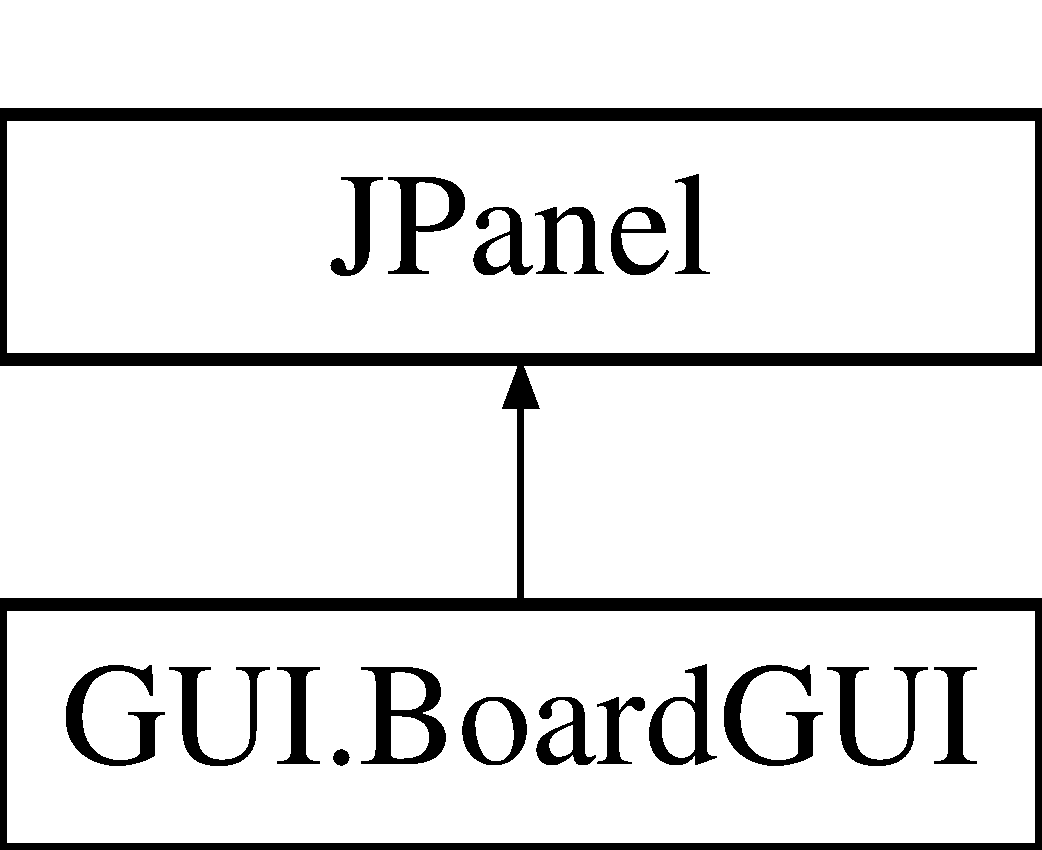
\includegraphics[height=2.000000cm]{class_g_u_i_1_1_board_g_u_i}
\end{center}
\end{figure}
\subsection*{Public Member Functions}
\begin{DoxyCompactItemize}
\item 
\mbox{\Hypertarget{class_g_u_i_1_1_board_g_u_i_a56dd455759059ad5efa9cfcc6d20cc90}\label{class_g_u_i_1_1_board_g_u_i_a56dd455759059ad5efa9cfcc6d20cc90}} 
void {\bfseries set\+Piece\+Initial} ()
\end{DoxyCompactItemize}
\subsection*{Public Attributes}
\begin{DoxyCompactItemize}
\item 
\mbox{\Hypertarget{class_g_u_i_1_1_board_g_u_i_a8ba06c3f4e942afd4e173c6d3919cd1b}\label{class_g_u_i_1_1_board_g_u_i_a8ba06c3f4e942afd4e173c6d3919cd1b}} 
\mbox{\hyperlink{class_g_u_i_1_1_button}{Button}} \mbox{[}$\,$\mbox{]}\mbox{[}$\,$\mbox{]} {\bfseries grids}
\end{DoxyCompactItemize}


The documentation for this class was generated from the following file\+:\begin{DoxyCompactItemize}
\item 
src/\+G\+U\+I/Board\+G\+U\+I.\+java\end{DoxyCompactItemize}

\hypertarget{class_g_u_i_1_1_button}{}\section{G\+U\+I.\+Button Class Reference}
\label{class_g_u_i_1_1_button}\index{G\+U\+I.\+Button@{G\+U\+I.\+Button}}
Inheritance diagram for G\+U\+I.\+Button\+:\begin{figure}[H]
\begin{center}
\leavevmode
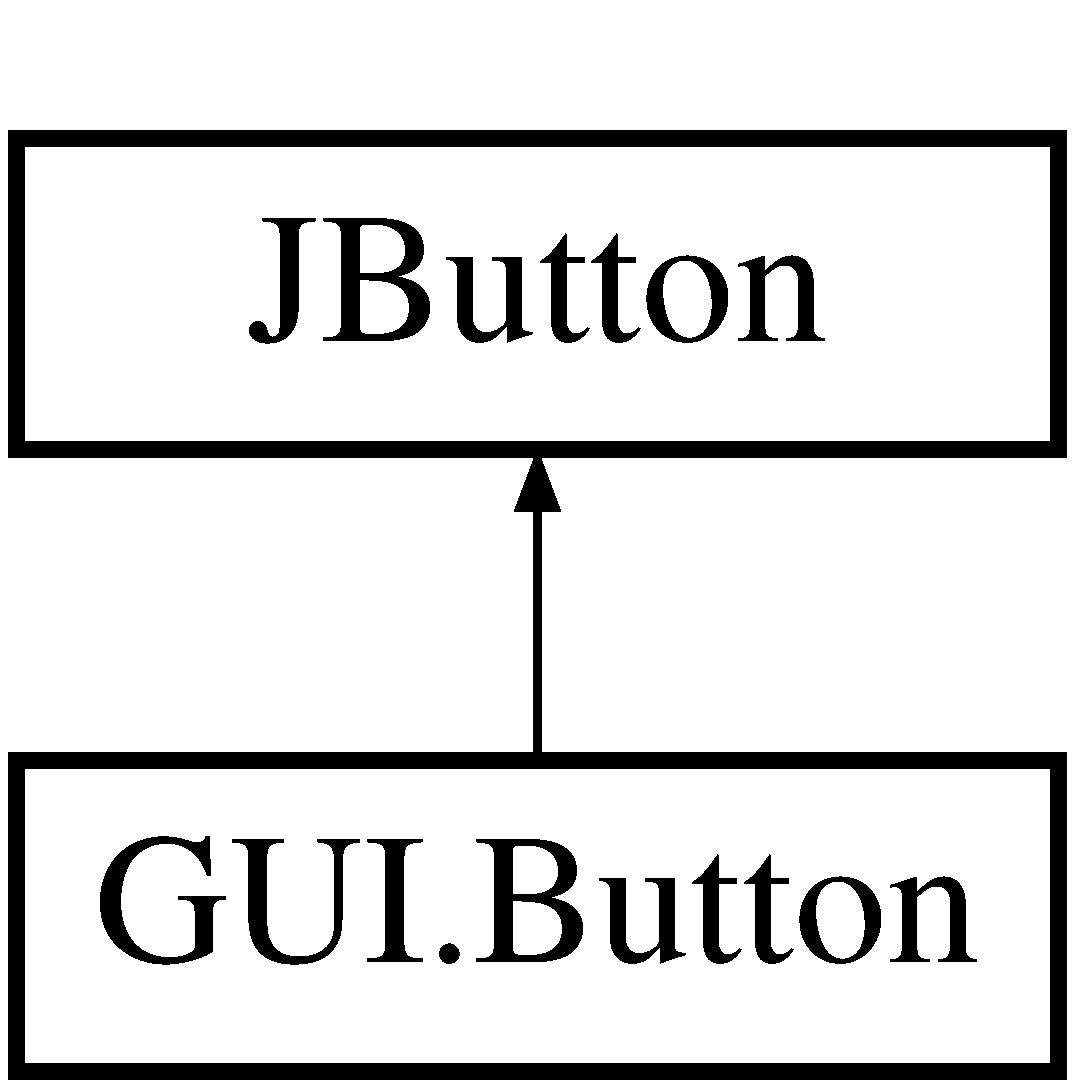
\includegraphics[height=2.000000cm]{class_g_u_i_1_1_button}
\end{center}
\end{figure}
\subsection*{Public Member Functions}
\begin{DoxyCompactItemize}
\item 
\mbox{\Hypertarget{class_g_u_i_1_1_button_a2fac288b37b1eb75e10f6f66d5f1f5b1}\label{class_g_u_i_1_1_button_a2fac288b37b1eb75e10f6f66d5f1f5b1}} 
{\bfseries Button} (int x, int y)
\end{DoxyCompactItemize}
\subsection*{Public Attributes}
\begin{DoxyCompactItemize}
\item 
\mbox{\Hypertarget{class_g_u_i_1_1_button_a8af19e5ff4096a6a61963d36675a55f2}\label{class_g_u_i_1_1_button_a8af19e5ff4096a6a61963d36675a55f2}} 
int {\bfseries x}
\item 
\mbox{\Hypertarget{class_g_u_i_1_1_button_ae0db1e73886a914b11dcabd2584404dc}\label{class_g_u_i_1_1_button_ae0db1e73886a914b11dcabd2584404dc}} 
int {\bfseries y}
\end{DoxyCompactItemize}


The documentation for this class was generated from the following file\+:\begin{DoxyCompactItemize}
\item 
src/\+G\+U\+I/Button.\+java\end{DoxyCompactItemize}

\hypertarget{classgame_1_1_game}{}\section{game.\+Game Class Reference}
\label{classgame_1_1_game}\index{game.\+Game@{game.\+Game}}
\subsection*{Public Member Functions}
\begin{DoxyCompactItemize}
\item 
\mbox{\hyperlink{classgame_1_1_game_add3e226871fd6c2b2e9b2f2d4cee4e94}{Game}} (int \mbox{\hyperlink{classgame_1_1_game_a7b89934f8f5f80ac47eb7b55f643d081}{rank}}, int \mbox{\hyperlink{classgame_1_1_game_ae0ed20be94f9ee5b87550ae2576ce891}{file}})
\item 
boolean \mbox{\hyperlink{classgame_1_1_game_a4020b63689c4aaaa1b67dc458ff2fbee}{judge}} (\mbox{\hyperlink{classgame_1_1_player}{Player}} moving, \mbox{\hyperlink{classgame_1_1_player}{Player}} standing)
\item 
boolean \mbox{\hyperlink{classgame_1_1_game_a7f87abb7baa5fa13ac53da8f534f79bd}{start}} ()
\end{DoxyCompactItemize}
\subsection*{Public Attributes}
\begin{DoxyCompactItemize}
\item 
\mbox{\hyperlink{classgame_1_1_player}{Player}} \mbox{\hyperlink{classgame_1_1_game_a28888dea5fdb92292566492315e4d27b}{player0}}
\item 
\mbox{\hyperlink{classgame_1_1_player}{Player}} \mbox{\hyperlink{classgame_1_1_game_ae4a1dc482dba322c7a5d3955efe01c81}{player1}}
\item 
\mbox{\hyperlink{classgame_1_1_board}{Board}} \mbox{\hyperlink{classgame_1_1_game_ae5a12a35960e274e9eac5ac382beb1b3}{play\+Board}}
\item 
int \mbox{\hyperlink{classgame_1_1_game_a7b89934f8f5f80ac47eb7b55f643d081}{rank}}
\item 
int \mbox{\hyperlink{classgame_1_1_game_ae0ed20be94f9ee5b87550ae2576ce891}{file}}
\end{DoxyCompactItemize}


\subsection{Constructor \& Destructor Documentation}
\mbox{\Hypertarget{classgame_1_1_game_add3e226871fd6c2b2e9b2f2d4cee4e94}\label{classgame_1_1_game_add3e226871fd6c2b2e9b2f2d4cee4e94}} 
\index{game\+::\+Game@{game\+::\+Game}!Game@{Game}}
\index{Game@{Game}!game\+::\+Game@{game\+::\+Game}}
\subsubsection{\texorpdfstring{Game()}{Game()}}
{\footnotesize\ttfamily game.\+Game.\+Game (\begin{DoxyParamCaption}\item[{int}]{rank,  }\item[{int}]{file }\end{DoxyParamCaption})\hspace{0.3cm}{\ttfamily [inline]}}

initialize game attributes 
\begin{DoxyParams}{Parameters}
{\em rank} & the number of rank on the board \\
\hline
{\em file} & the number of file on the board \\
\hline
\end{DoxyParams}


\subsection{Member Function Documentation}
\mbox{\Hypertarget{classgame_1_1_game_a4020b63689c4aaaa1b67dc458ff2fbee}\label{classgame_1_1_game_a4020b63689c4aaaa1b67dc458ff2fbee}} 
\index{game\+::\+Game@{game\+::\+Game}!judge@{judge}}
\index{judge@{judge}!game\+::\+Game@{game\+::\+Game}}
\subsubsection{\texorpdfstring{judge()}{judge()}}
{\footnotesize\ttfamily boolean game.\+Game.\+judge (\begin{DoxyParamCaption}\item[{\mbox{\hyperlink{classgame_1_1_player}{Player}}}]{moving,  }\item[{\mbox{\hyperlink{classgame_1_1_player}{Player}}}]{standing }\end{DoxyParamCaption})\hspace{0.3cm}{\ttfamily [inline]}}

judge whether the game should end checkmate or stalemate happens 
\begin{DoxyParams}{Parameters}
{\em moving} & player for this turn \\
\hline
{\em standing} & player who is waiting for next turn \\
\hline
\end{DoxyParams}
\mbox{\Hypertarget{classgame_1_1_game_a7f87abb7baa5fa13ac53da8f534f79bd}\label{classgame_1_1_game_a7f87abb7baa5fa13ac53da8f534f79bd}} 
\index{game\+::\+Game@{game\+::\+Game}!start@{start}}
\index{start@{start}!game\+::\+Game@{game\+::\+Game}}
\subsubsection{\texorpdfstring{start()}{start()}}
{\footnotesize\ttfamily boolean game.\+Game.\+start (\begin{DoxyParamCaption}{ }\end{DoxyParamCaption})\hspace{0.3cm}{\ttfamily [inline]}}

game start interface \begin{DoxyReturn}{Returns}
whether game is end 
\end{DoxyReturn}


\subsection{Member Data Documentation}
\mbox{\Hypertarget{classgame_1_1_game_ae0ed20be94f9ee5b87550ae2576ce891}\label{classgame_1_1_game_ae0ed20be94f9ee5b87550ae2576ce891}} 
\index{game\+::\+Game@{game\+::\+Game}!file@{file}}
\index{file@{file}!game\+::\+Game@{game\+::\+Game}}
\subsubsection{\texorpdfstring{file}{file}}
{\footnotesize\ttfamily int game.\+Game.\+file}

the number of file on the board \mbox{\Hypertarget{classgame_1_1_game_ae5a12a35960e274e9eac5ac382beb1b3}\label{classgame_1_1_game_ae5a12a35960e274e9eac5ac382beb1b3}} 
\index{game\+::\+Game@{game\+::\+Game}!play\+Board@{play\+Board}}
\index{play\+Board@{play\+Board}!game\+::\+Game@{game\+::\+Game}}
\subsubsection{\texorpdfstring{play\+Board}{playBoard}}
{\footnotesize\ttfamily \mbox{\hyperlink{classgame_1_1_board}{Board}} game.\+Game.\+play\+Board}

the board for this game \mbox{\Hypertarget{classgame_1_1_game_a28888dea5fdb92292566492315e4d27b}\label{classgame_1_1_game_a28888dea5fdb92292566492315e4d27b}} 
\index{game\+::\+Game@{game\+::\+Game}!player0@{player0}}
\index{player0@{player0}!game\+::\+Game@{game\+::\+Game}}
\subsubsection{\texorpdfstring{player0}{player0}}
{\footnotesize\ttfamily \mbox{\hyperlink{classgame_1_1_player}{Player}} game.\+Game.\+player0}

the upper player \mbox{\Hypertarget{classgame_1_1_game_ae4a1dc482dba322c7a5d3955efe01c81}\label{classgame_1_1_game_ae4a1dc482dba322c7a5d3955efe01c81}} 
\index{game\+::\+Game@{game\+::\+Game}!player1@{player1}}
\index{player1@{player1}!game\+::\+Game@{game\+::\+Game}}
\subsubsection{\texorpdfstring{player1}{player1}}
{\footnotesize\ttfamily \mbox{\hyperlink{classgame_1_1_player}{Player}} game.\+Game.\+player1}

the player locates downward \mbox{\Hypertarget{classgame_1_1_game_a7b89934f8f5f80ac47eb7b55f643d081}\label{classgame_1_1_game_a7b89934f8f5f80ac47eb7b55f643d081}} 
\index{game\+::\+Game@{game\+::\+Game}!rank@{rank}}
\index{rank@{rank}!game\+::\+Game@{game\+::\+Game}}
\subsubsection{\texorpdfstring{rank}{rank}}
{\footnotesize\ttfamily int game.\+Game.\+rank}

the number of rank on the board 

The documentation for this class was generated from the following file\+:\begin{DoxyCompactItemize}
\item 
src/game/Game.\+java\end{DoxyCompactItemize}

\hypertarget{class_g_u_i_1_1_game_g_u_i}{}\section{G\+U\+I.\+Game\+G\+UI Class Reference}
\label{class_g_u_i_1_1_game_g_u_i}\index{G\+U\+I.\+Game\+G\+UI@{G\+U\+I.\+Game\+G\+UI}}
\subsection*{Static Public Member Functions}
\begin{DoxyCompactItemize}
\item 
\mbox{\Hypertarget{class_g_u_i_1_1_game_g_u_i_ac538a171ff001d8f4b2bca9c37e4a7f8}\label{class_g_u_i_1_1_game_g_u_i_ac538a171ff001d8f4b2bca9c37e4a7f8}} 
static void {\bfseries main} (String\mbox{[}$\,$\mbox{]} args)
\end{DoxyCompactItemize}


The documentation for this class was generated from the following file\+:\begin{DoxyCompactItemize}
\item 
src/\+G\+U\+I/Game\+G\+U\+I.\+java\end{DoxyCompactItemize}

\hypertarget{classpieces_1_1_hopper}{}\section{pieces.\+Hopper Class Reference}
\label{classpieces_1_1_hopper}\index{pieces.\+Hopper@{pieces.\+Hopper}}
Inheritance diagram for pieces.\+Hopper\+:\begin{figure}[H]
\begin{center}
\leavevmode
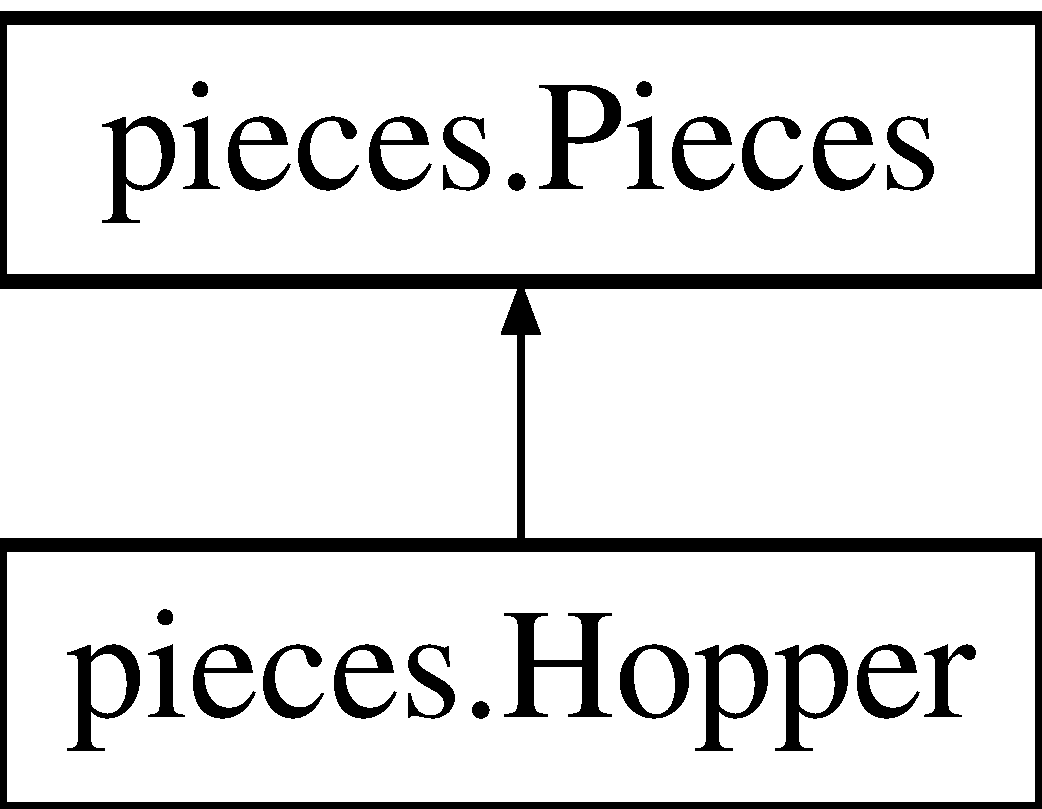
\includegraphics[height=2.000000cm]{classpieces_1_1_hopper}
\end{center}
\end{figure}
\subsection*{Public Member Functions}
\begin{DoxyCompactItemize}
\item 
\mbox{\hyperlink{classpieces_1_1_hopper_a61251ca61d7a92fcfbaa12b6110e02e8}{Hopper}} (int \mbox{\hyperlink{classpieces_1_1_pieces_ac5178f9b8a6b0c4235851475081249f3}{x}}, int \mbox{\hyperlink{classpieces_1_1_pieces_a66d911734967a8ced1b9792fe900fadb}{y}}, \mbox{\hyperlink{classgame_1_1_player}{Player}} \mbox{\hyperlink{classpieces_1_1_pieces_a49f35044dd36e5c4b04261a8ea54ad0c}{player}}, \mbox{\hyperlink{classgame_1_1_board}{Board}} play\+Board)
\item 
boolean \mbox{\hyperlink{classpieces_1_1_hopper_a74ab407bf1ef68867f2f06f68ad73f06}{is\+Valid\+Move}} (int newX, int newY)
\item 
List$<$ int\mbox{[}$\,$\mbox{]}$>$ \mbox{\hyperlink{classpieces_1_1_hopper_a9cb2384553aded22be588ae1eff76d09}{moving}} (int newX, int newY)
\end{DoxyCompactItemize}
\subsection*{Additional Inherited Members}


\subsection{Detailed Description}
\mbox{\hyperlink{classpieces_1_1_hopper}{Hopper}} class 

\mbox{\hyperlink{classpieces_1_1_hopper}{Hopper}} moves by jumping over its direct piece, \mbox{\hyperlink{classpieces_1_1_hopper}{Hopper}} only jump to its forward, backward, left and right direction, \mbox{\hyperlink{classpieces_1_1_hopper}{Hopper}} can only jump once each time. 

\subsection{Constructor \& Destructor Documentation}
\mbox{\Hypertarget{classpieces_1_1_hopper_a61251ca61d7a92fcfbaa12b6110e02e8}\label{classpieces_1_1_hopper_a61251ca61d7a92fcfbaa12b6110e02e8}} 
\index{pieces\+::\+Hopper@{pieces\+::\+Hopper}!Hopper@{Hopper}}
\index{Hopper@{Hopper}!pieces\+::\+Hopper@{pieces\+::\+Hopper}}
\subsubsection{\texorpdfstring{Hopper()}{Hopper()}}
{\footnotesize\ttfamily pieces.\+Hopper.\+Hopper (\begin{DoxyParamCaption}\item[{int}]{x,  }\item[{int}]{y,  }\item[{\mbox{\hyperlink{classgame_1_1_player}{Player}}}]{player,  }\item[{\mbox{\hyperlink{classgame_1_1_board}{Board}}}]{play\+Board }\end{DoxyParamCaption})\hspace{0.3cm}{\ttfamily [inline]}}

initialize hopper attributes 
\begin{DoxyParams}{Parameters}
{\em x} & the initial rank position \\
\hline
{\em y} & the initial file position \\
\hline
{\em player} & the player piece belong to \\
\hline
\end{DoxyParams}


\subsection{Member Function Documentation}
\mbox{\Hypertarget{classpieces_1_1_hopper_a74ab407bf1ef68867f2f06f68ad73f06}\label{classpieces_1_1_hopper_a74ab407bf1ef68867f2f06f68ad73f06}} 
\index{pieces\+::\+Hopper@{pieces\+::\+Hopper}!is\+Valid\+Move@{is\+Valid\+Move}}
\index{is\+Valid\+Move@{is\+Valid\+Move}!pieces\+::\+Hopper@{pieces\+::\+Hopper}}
\subsubsection{\texorpdfstring{is\+Valid\+Move()}{isValidMove()}}
{\footnotesize\ttfamily boolean pieces.\+Hopper.\+is\+Valid\+Move (\begin{DoxyParamCaption}\item[{int}]{newX,  }\item[{int}]{newY }\end{DoxyParamCaption})\hspace{0.3cm}{\ttfamily [inline]}}

check whether hopper is moved by its own rule, hopper can at most move two squares each time 
\begin{DoxyParams}{Parameters}
{\em newX} & destination rank of the piece \\
\hline
{\em newY} & destination file of the piece \\
\hline
\end{DoxyParams}
\begin{DoxyReturn}{Returns}
whether this step is a valid move 
\end{DoxyReturn}
\mbox{\Hypertarget{classpieces_1_1_hopper_a9cb2384553aded22be588ae1eff76d09}\label{classpieces_1_1_hopper_a9cb2384553aded22be588ae1eff76d09}} 
\index{pieces\+::\+Hopper@{pieces\+::\+Hopper}!moving@{moving}}
\index{moving@{moving}!pieces\+::\+Hopper@{pieces\+::\+Hopper}}
\subsubsection{\texorpdfstring{moving()}{moving()}}
{\footnotesize\ttfamily List$<$int\mbox{[}$\,$\mbox{]}$>$ pieces.\+Hopper.\+moving (\begin{DoxyParamCaption}\item[{int}]{newX,  }\item[{int}]{newY }\end{DoxyParamCaption})\hspace{0.3cm}{\ttfamily [inline]}}

store the passing positions a helper function for later check leap over other pieces 
\begin{DoxyParams}{Parameters}
{\em newX} & destination rank of the piece \\
\hline
{\em newY} & destination file of the piece \\
\hline
\end{DoxyParams}
\begin{DoxyReturn}{Returns}
a null array, since hopper must leap over one piece 
\end{DoxyReturn}


The documentation for this class was generated from the following file\+:\begin{DoxyCompactItemize}
\item 
src/pieces/Hopper.\+java\end{DoxyCompactItemize}

\hypertarget{classpieces_1_1_king}{}\section{pieces.\+King Class Reference}
\label{classpieces_1_1_king}\index{pieces.\+King@{pieces.\+King}}
Inheritance diagram for pieces.\+King\+:\begin{figure}[H]
\begin{center}
\leavevmode
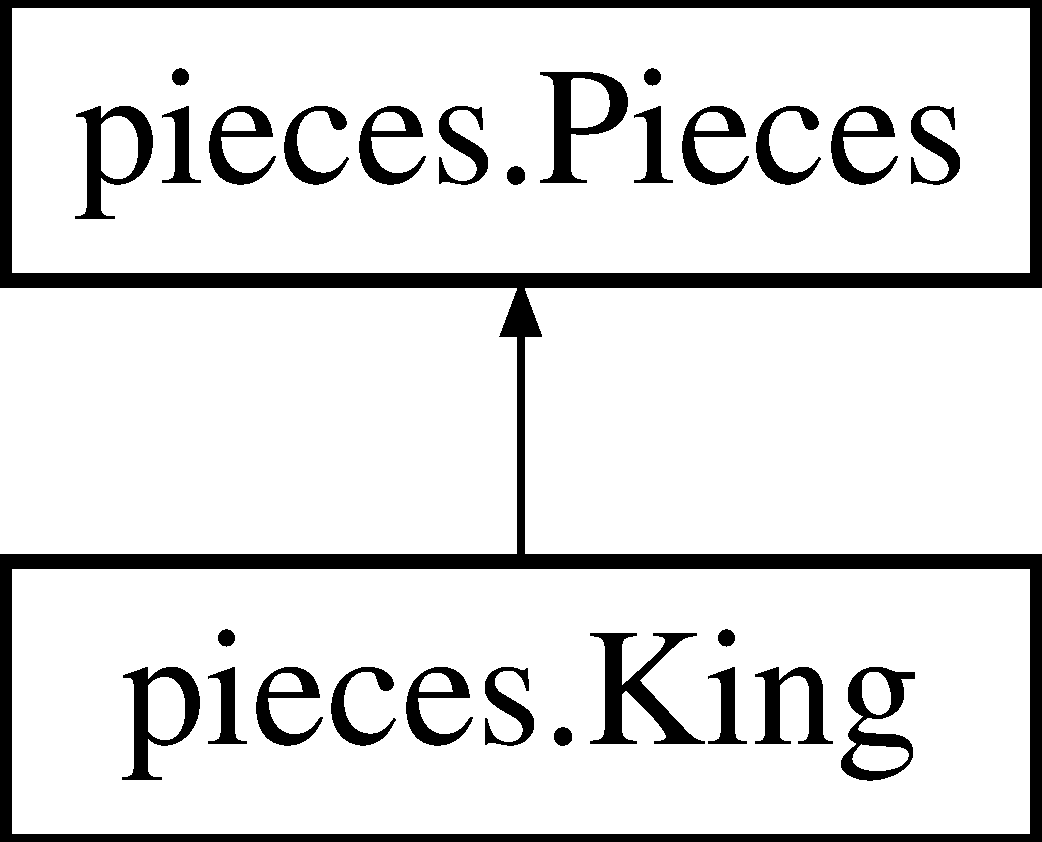
\includegraphics[height=2.000000cm]{classpieces_1_1_king}
\end{center}
\end{figure}
\subsection*{Public Member Functions}
\begin{DoxyCompactItemize}
\item 
\mbox{\hyperlink{classpieces_1_1_king_aeb8f844df907887869024c67508ab8f0}{King}} (int \mbox{\hyperlink{classpieces_1_1_pieces_ac5178f9b8a6b0c4235851475081249f3}{x}}, int \mbox{\hyperlink{classpieces_1_1_pieces_a66d911734967a8ced1b9792fe900fadb}{y}}, \mbox{\hyperlink{classgame_1_1_player}{Player}} \mbox{\hyperlink{classpieces_1_1_pieces_a49f35044dd36e5c4b04261a8ea54ad0c}{player}})
\item 
boolean \mbox{\hyperlink{classpieces_1_1_king_a308ed50d558d0c681242c8dcd76cd37e}{is\+Valid\+Move}} (int newX, int newY)
\item 
List$<$ int\mbox{[}$\,$\mbox{]}$>$ \mbox{\hyperlink{classpieces_1_1_king_a8cadd535c0a47713806bb65c975f2233}{moving}} (int newX, int newY)
\end{DoxyCompactItemize}
\subsection*{Additional Inherited Members}


\subsection{Detailed Description}
\mbox{\hyperlink{classpieces_1_1_king}{King}} class 

The king moves one square in any direction. 

\subsection{Constructor \& Destructor Documentation}
\mbox{\Hypertarget{classpieces_1_1_king_aeb8f844df907887869024c67508ab8f0}\label{classpieces_1_1_king_aeb8f844df907887869024c67508ab8f0}} 
\index{pieces\+::\+King@{pieces\+::\+King}!King@{King}}
\index{King@{King}!pieces\+::\+King@{pieces\+::\+King}}
\subsubsection{\texorpdfstring{King()}{King()}}
{\footnotesize\ttfamily pieces.\+King.\+King (\begin{DoxyParamCaption}\item[{int}]{x,  }\item[{int}]{y,  }\item[{\mbox{\hyperlink{classgame_1_1_player}{Player}}}]{player }\end{DoxyParamCaption})\hspace{0.3cm}{\ttfamily [inline]}}

initialize king attributes 
\begin{DoxyParams}{Parameters}
{\em x} & the initial rank position \\
\hline
{\em y} & the initial file position \\
\hline
{\em player} & the player piece belong to \\
\hline
\end{DoxyParams}


\subsection{Member Function Documentation}
\mbox{\Hypertarget{classpieces_1_1_king_a308ed50d558d0c681242c8dcd76cd37e}\label{classpieces_1_1_king_a308ed50d558d0c681242c8dcd76cd37e}} 
\index{pieces\+::\+King@{pieces\+::\+King}!is\+Valid\+Move@{is\+Valid\+Move}}
\index{is\+Valid\+Move@{is\+Valid\+Move}!pieces\+::\+King@{pieces\+::\+King}}
\subsubsection{\texorpdfstring{is\+Valid\+Move()}{isValidMove()}}
{\footnotesize\ttfamily boolean pieces.\+King.\+is\+Valid\+Move (\begin{DoxyParamCaption}\item[{int}]{newX,  }\item[{int}]{newY }\end{DoxyParamCaption})\hspace{0.3cm}{\ttfamily [inline]}}

check whether king is moved by its own rule; king could only move one step but can in all directions 
\begin{DoxyParams}{Parameters}
{\em newX} & destination rank of the piece \\
\hline
{\em newY} & destination file of the piece \\
\hline
\end{DoxyParams}
\begin{DoxyReturn}{Returns}
whether this step is a valid move 
\end{DoxyReturn}
\mbox{\Hypertarget{classpieces_1_1_king_a8cadd535c0a47713806bb65c975f2233}\label{classpieces_1_1_king_a8cadd535c0a47713806bb65c975f2233}} 
\index{pieces\+::\+King@{pieces\+::\+King}!moving@{moving}}
\index{moving@{moving}!pieces\+::\+King@{pieces\+::\+King}}
\subsubsection{\texorpdfstring{moving()}{moving()}}
{\footnotesize\ttfamily List$<$int\mbox{[}$\,$\mbox{]}$>$ pieces.\+King.\+moving (\begin{DoxyParamCaption}\item[{int}]{newX,  }\item[{int}]{newY }\end{DoxyParamCaption})\hspace{0.3cm}{\ttfamily [inline]}}

store the passing positions a helper function for later check leap over other pieces 
\begin{DoxyParams}{Parameters}
{\em newX} & destination rank of the piece \\
\hline
{\em newY} & destination file of the piece \\
\hline
\end{DoxyParams}
\begin{DoxyReturn}{Returns}
since king only move one step, there\textquotesingle{}s no square to leap over 
\end{DoxyReturn}


The documentation for this class was generated from the following file\+:\begin{DoxyCompactItemize}
\item 
src/pieces/King.\+java\end{DoxyCompactItemize}

\hypertarget{classpieces_1_1_knight}{}\section{pieces.\+Knight Class Reference}
\label{classpieces_1_1_knight}\index{pieces.\+Knight@{pieces.\+Knight}}
Inheritance diagram for pieces.\+Knight\+:\begin{figure}[H]
\begin{center}
\leavevmode
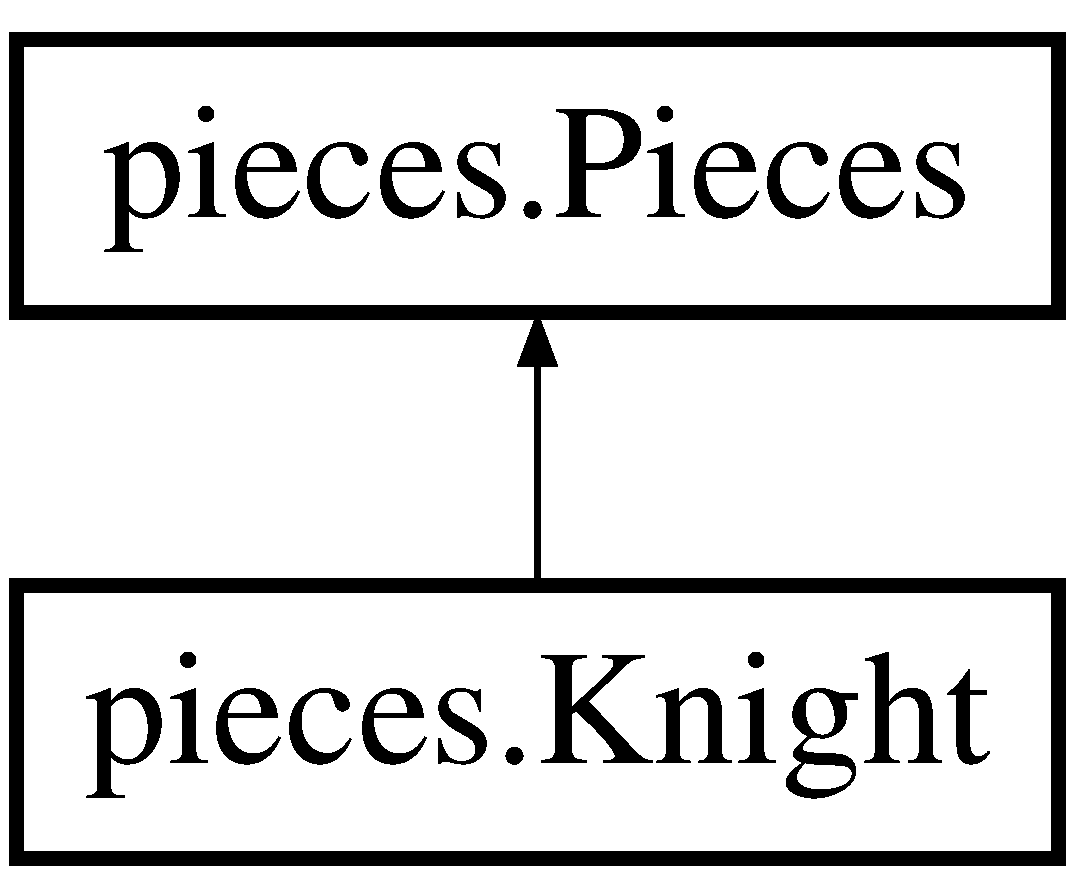
\includegraphics[height=2.000000cm]{classpieces_1_1_knight}
\end{center}
\end{figure}
\subsection*{Public Member Functions}
\begin{DoxyCompactItemize}
\item 
\mbox{\hyperlink{classpieces_1_1_knight_a90125366cf56f2bda5c94e75d68c6f07}{Knight}} (int \mbox{\hyperlink{classpieces_1_1_pieces_ac5178f9b8a6b0c4235851475081249f3}{x}}, int \mbox{\hyperlink{classpieces_1_1_pieces_a66d911734967a8ced1b9792fe900fadb}{y}}, \mbox{\hyperlink{classgame_1_1_player}{Player}} \mbox{\hyperlink{classpieces_1_1_pieces_a49f35044dd36e5c4b04261a8ea54ad0c}{player}})
\item 
boolean \mbox{\hyperlink{classpieces_1_1_knight_a3c379a4a0fe48e0f066de58a9b2b236d}{is\+Valid\+Move}} (int newX, int newY)
\item 
List$<$ int\mbox{[}$\,$\mbox{]}$>$ \mbox{\hyperlink{classpieces_1_1_knight_ab70ead116fdcb7786b07b671639b792e}{moving}} (int newX, int newY)
\end{DoxyCompactItemize}
\subsection*{Additional Inherited Members}


\subsection{Detailed Description}
\mbox{\hyperlink{classpieces_1_1_knight}{Knight}} class 

The knight moves to any of the closest squares that are not on the same rank, file, or diagonal, thus the move forms an \char`\"{}\+L\char`\"{}-\/shape\+: two squares vertically and one square horizontally, or two squares horizontally and one square vertically. The knight is the only piece that can leap over other pieces. 

\subsection{Constructor \& Destructor Documentation}
\mbox{\Hypertarget{classpieces_1_1_knight_a90125366cf56f2bda5c94e75d68c6f07}\label{classpieces_1_1_knight_a90125366cf56f2bda5c94e75d68c6f07}} 
\index{pieces\+::\+Knight@{pieces\+::\+Knight}!Knight@{Knight}}
\index{Knight@{Knight}!pieces\+::\+Knight@{pieces\+::\+Knight}}
\subsubsection{\texorpdfstring{Knight()}{Knight()}}
{\footnotesize\ttfamily pieces.\+Knight.\+Knight (\begin{DoxyParamCaption}\item[{int}]{x,  }\item[{int}]{y,  }\item[{\mbox{\hyperlink{classgame_1_1_player}{Player}}}]{player }\end{DoxyParamCaption})\hspace{0.3cm}{\ttfamily [inline]}}

initialize knight attributes 
\begin{DoxyParams}{Parameters}
{\em x} & the initial rank position \\
\hline
{\em y} & the initial file position \\
\hline
{\em player} & the player piece belong to \\
\hline
\end{DoxyParams}


\subsection{Member Function Documentation}
\mbox{\Hypertarget{classpieces_1_1_knight_a3c379a4a0fe48e0f066de58a9b2b236d}\label{classpieces_1_1_knight_a3c379a4a0fe48e0f066de58a9b2b236d}} 
\index{pieces\+::\+Knight@{pieces\+::\+Knight}!is\+Valid\+Move@{is\+Valid\+Move}}
\index{is\+Valid\+Move@{is\+Valid\+Move}!pieces\+::\+Knight@{pieces\+::\+Knight}}
\subsubsection{\texorpdfstring{is\+Valid\+Move()}{isValidMove()}}
{\footnotesize\ttfamily boolean pieces.\+Knight.\+is\+Valid\+Move (\begin{DoxyParamCaption}\item[{int}]{newX,  }\item[{int}]{newY }\end{DoxyParamCaption})\hspace{0.3cm}{\ttfamily [inline]}}

check whether knight is moved by its own rule; knight could only move in \textquotesingle{}L\textquotesingle{} way 
\begin{DoxyParams}{Parameters}
{\em newX} & destination rank of the piece \\
\hline
{\em newY} & destination file of the piece \\
\hline
\end{DoxyParams}
\begin{DoxyReturn}{Returns}
whether this step is a valid move 
\end{DoxyReturn}
\mbox{\Hypertarget{classpieces_1_1_knight_ab70ead116fdcb7786b07b671639b792e}\label{classpieces_1_1_knight_ab70ead116fdcb7786b07b671639b792e}} 
\index{pieces\+::\+Knight@{pieces\+::\+Knight}!moving@{moving}}
\index{moving@{moving}!pieces\+::\+Knight@{pieces\+::\+Knight}}
\subsubsection{\texorpdfstring{moving()}{moving()}}
{\footnotesize\ttfamily List$<$int\mbox{[}$\,$\mbox{]}$>$ pieces.\+Knight.\+moving (\begin{DoxyParamCaption}\item[{int}]{newX,  }\item[{int}]{newY }\end{DoxyParamCaption})\hspace{0.3cm}{\ttfamily [inline]}}

store the passing positions a helper function for later check leap over other pieces 
\begin{DoxyParams}{Parameters}
{\em newX} & destination rank of the piece \\
\hline
{\em newY} & destination file of the piece \\
\hline
\end{DoxyParams}
\begin{DoxyReturn}{Returns}
knight can leap over other pieces, so return an empty list 
\end{DoxyReturn}


The documentation for this class was generated from the following file\+:\begin{DoxyCompactItemize}
\item 
src/pieces/Knight.\+java\end{DoxyCompactItemize}

\hypertarget{classpieces_1_1_pawn}{}\section{pieces.\+Pawn Class Reference}
\label{classpieces_1_1_pawn}\index{pieces.\+Pawn@{pieces.\+Pawn}}
Inheritance diagram for pieces.\+Pawn\+:\begin{figure}[H]
\begin{center}
\leavevmode
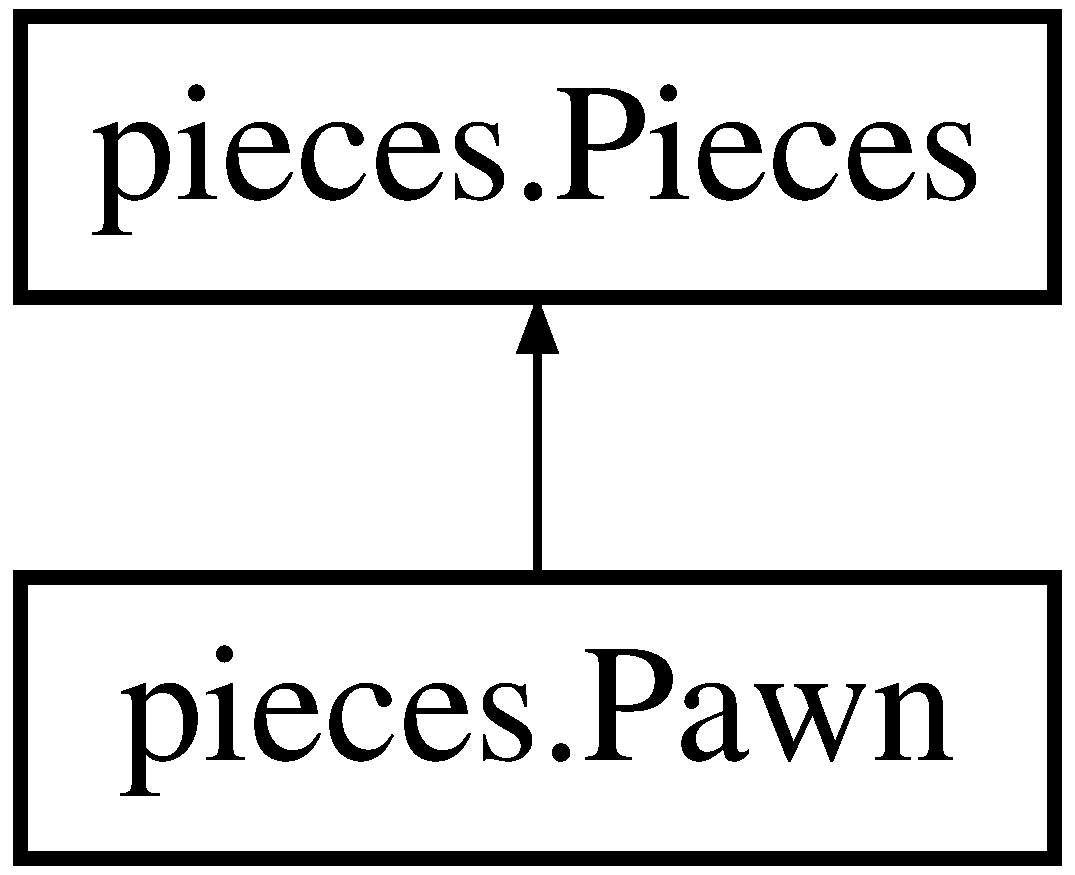
\includegraphics[height=2.000000cm]{classpieces_1_1_pawn}
\end{center}
\end{figure}
\subsection*{Public Member Functions}
\begin{DoxyCompactItemize}
\item 
\mbox{\hyperlink{classpieces_1_1_pawn_ac5014277fafcc4556c3816123a353540}{Pawn}} (int \mbox{\hyperlink{classpieces_1_1_pieces_ac5178f9b8a6b0c4235851475081249f3}{x}}, int \mbox{\hyperlink{classpieces_1_1_pieces_a66d911734967a8ced1b9792fe900fadb}{y}}, \mbox{\hyperlink{classgame_1_1_player}{Player}} \mbox{\hyperlink{classpieces_1_1_pieces_a49f35044dd36e5c4b04261a8ea54ad0c}{player}}, \mbox{\hyperlink{classgame_1_1_board}{Board}} play\+Board)
\item 
boolean \mbox{\hyperlink{classpieces_1_1_pawn_a16fd663948369962794e5d278f3f8107}{is\+Valid\+Move}} (int newX, int newY)
\item 
List$<$ int\mbox{[}$\,$\mbox{]}$>$ \mbox{\hyperlink{classpieces_1_1_pawn_a2d97ee355c63d23a5ff0117ddf2a85b9}{moving}} (int newX, int newY)
\item 
void \mbox{\hyperlink{classpieces_1_1_pawn_ae20b1ede53cd4d2f6c1c064d05efaf93}{move}} (int newX, int newY)
\end{DoxyCompactItemize}
\subsection*{Additional Inherited Members}


\subsection{Detailed Description}
\mbox{\hyperlink{classpieces_1_1_pawn}{Pawn}} class 

The pawn may move forward to the unoccupied square immediately in front of it on the same file; or on its first move it may advance two squares along the same file provided both squares are unoccupied; or it may move to a square occupied by an opponent\textquotesingle{}s piece which is diagonally in front of it on an adjacent file, capturing that piece. 

\subsection{Constructor \& Destructor Documentation}
\mbox{\Hypertarget{classpieces_1_1_pawn_ac5014277fafcc4556c3816123a353540}\label{classpieces_1_1_pawn_ac5014277fafcc4556c3816123a353540}} 
\index{pieces\+::\+Pawn@{pieces\+::\+Pawn}!Pawn@{Pawn}}
\index{Pawn@{Pawn}!pieces\+::\+Pawn@{pieces\+::\+Pawn}}
\subsubsection{\texorpdfstring{Pawn()}{Pawn()}}
{\footnotesize\ttfamily pieces.\+Pawn.\+Pawn (\begin{DoxyParamCaption}\item[{int}]{x,  }\item[{int}]{y,  }\item[{\mbox{\hyperlink{classgame_1_1_player}{Player}}}]{player,  }\item[{\mbox{\hyperlink{classgame_1_1_board}{Board}}}]{play\+Board }\end{DoxyParamCaption})\hspace{0.3cm}{\ttfamily [inline]}}

initialize pawn attributes 
\begin{DoxyParams}{Parameters}
{\em x} & the initial rank position \\
\hline
{\em y} & the initial file position \\
\hline
{\em player} & the player piece belong to \\
\hline
\end{DoxyParams}


\subsection{Member Function Documentation}
\mbox{\Hypertarget{classpieces_1_1_pawn_a16fd663948369962794e5d278f3f8107}\label{classpieces_1_1_pawn_a16fd663948369962794e5d278f3f8107}} 
\index{pieces\+::\+Pawn@{pieces\+::\+Pawn}!is\+Valid\+Move@{is\+Valid\+Move}}
\index{is\+Valid\+Move@{is\+Valid\+Move}!pieces\+::\+Pawn@{pieces\+::\+Pawn}}
\subsubsection{\texorpdfstring{is\+Valid\+Move()}{isValidMove()}}
{\footnotesize\ttfamily boolean pieces.\+Pawn.\+is\+Valid\+Move (\begin{DoxyParamCaption}\item[{int}]{newX,  }\item[{int}]{newY }\end{DoxyParamCaption})\hspace{0.3cm}{\ttfamily [inline]}}

check whether pawn is moved by its own rule; pawn could only move forward, only one step except for the first move 
\begin{DoxyParams}{Parameters}
{\em newX} & newX destination rank of the piece \\
\hline
{\em newY} & destination file of the piece \\
\hline
\end{DoxyParams}
\begin{DoxyReturn}{Returns}
whether this step is a valid move 
\end{DoxyReturn}
\mbox{\Hypertarget{classpieces_1_1_pawn_ae20b1ede53cd4d2f6c1c064d05efaf93}\label{classpieces_1_1_pawn_ae20b1ede53cd4d2f6c1c064d05efaf93}} 
\index{pieces\+::\+Pawn@{pieces\+::\+Pawn}!move@{move}}
\index{move@{move}!pieces\+::\+Pawn@{pieces\+::\+Pawn}}
\subsubsection{\texorpdfstring{move()}{move()}}
{\footnotesize\ttfamily void pieces.\+Pawn.\+move (\begin{DoxyParamCaption}\item[{int}]{newX,  }\item[{int}]{newY }\end{DoxyParamCaption})\hspace{0.3cm}{\ttfamily [inline]}}

update the piece position 
\begin{DoxyParams}{Parameters}
{\em newX} & destination rank of the piece \\
\hline
{\em newY} & destination file of the piece \\
\hline
\end{DoxyParams}
\mbox{\Hypertarget{classpieces_1_1_pawn_a2d97ee355c63d23a5ff0117ddf2a85b9}\label{classpieces_1_1_pawn_a2d97ee355c63d23a5ff0117ddf2a85b9}} 
\index{pieces\+::\+Pawn@{pieces\+::\+Pawn}!moving@{moving}}
\index{moving@{moving}!pieces\+::\+Pawn@{pieces\+::\+Pawn}}
\subsubsection{\texorpdfstring{moving()}{moving()}}
{\footnotesize\ttfamily List$<$int\mbox{[}$\,$\mbox{]}$>$ pieces.\+Pawn.\+moving (\begin{DoxyParamCaption}\item[{int}]{newX,  }\item[{int}]{newY }\end{DoxyParamCaption})\hspace{0.3cm}{\ttfamily [inline]}}

store the passing positions a helper function for later check leap over other pieces 
\begin{DoxyParams}{Parameters}
{\em newX} & destination rank of the piece \\
\hline
{\em newY} & destination file of the piece \\
\hline
\end{DoxyParams}
\begin{DoxyReturn}{Returns}
only if pawn move two steps, we store the leaped over position 
\end{DoxyReturn}


The documentation for this class was generated from the following file\+:\begin{DoxyCompactItemize}
\item 
src/pieces/Pawn.\+java\end{DoxyCompactItemize}

\hypertarget{classpieces_1_1_pieces}{}\section{pieces.\+Pieces Class Reference}
\label{classpieces_1_1_pieces}\index{pieces.\+Pieces@{pieces.\+Pieces}}
Inheritance diagram for pieces.\+Pieces\+:\begin{figure}[H]
\begin{center}
\leavevmode
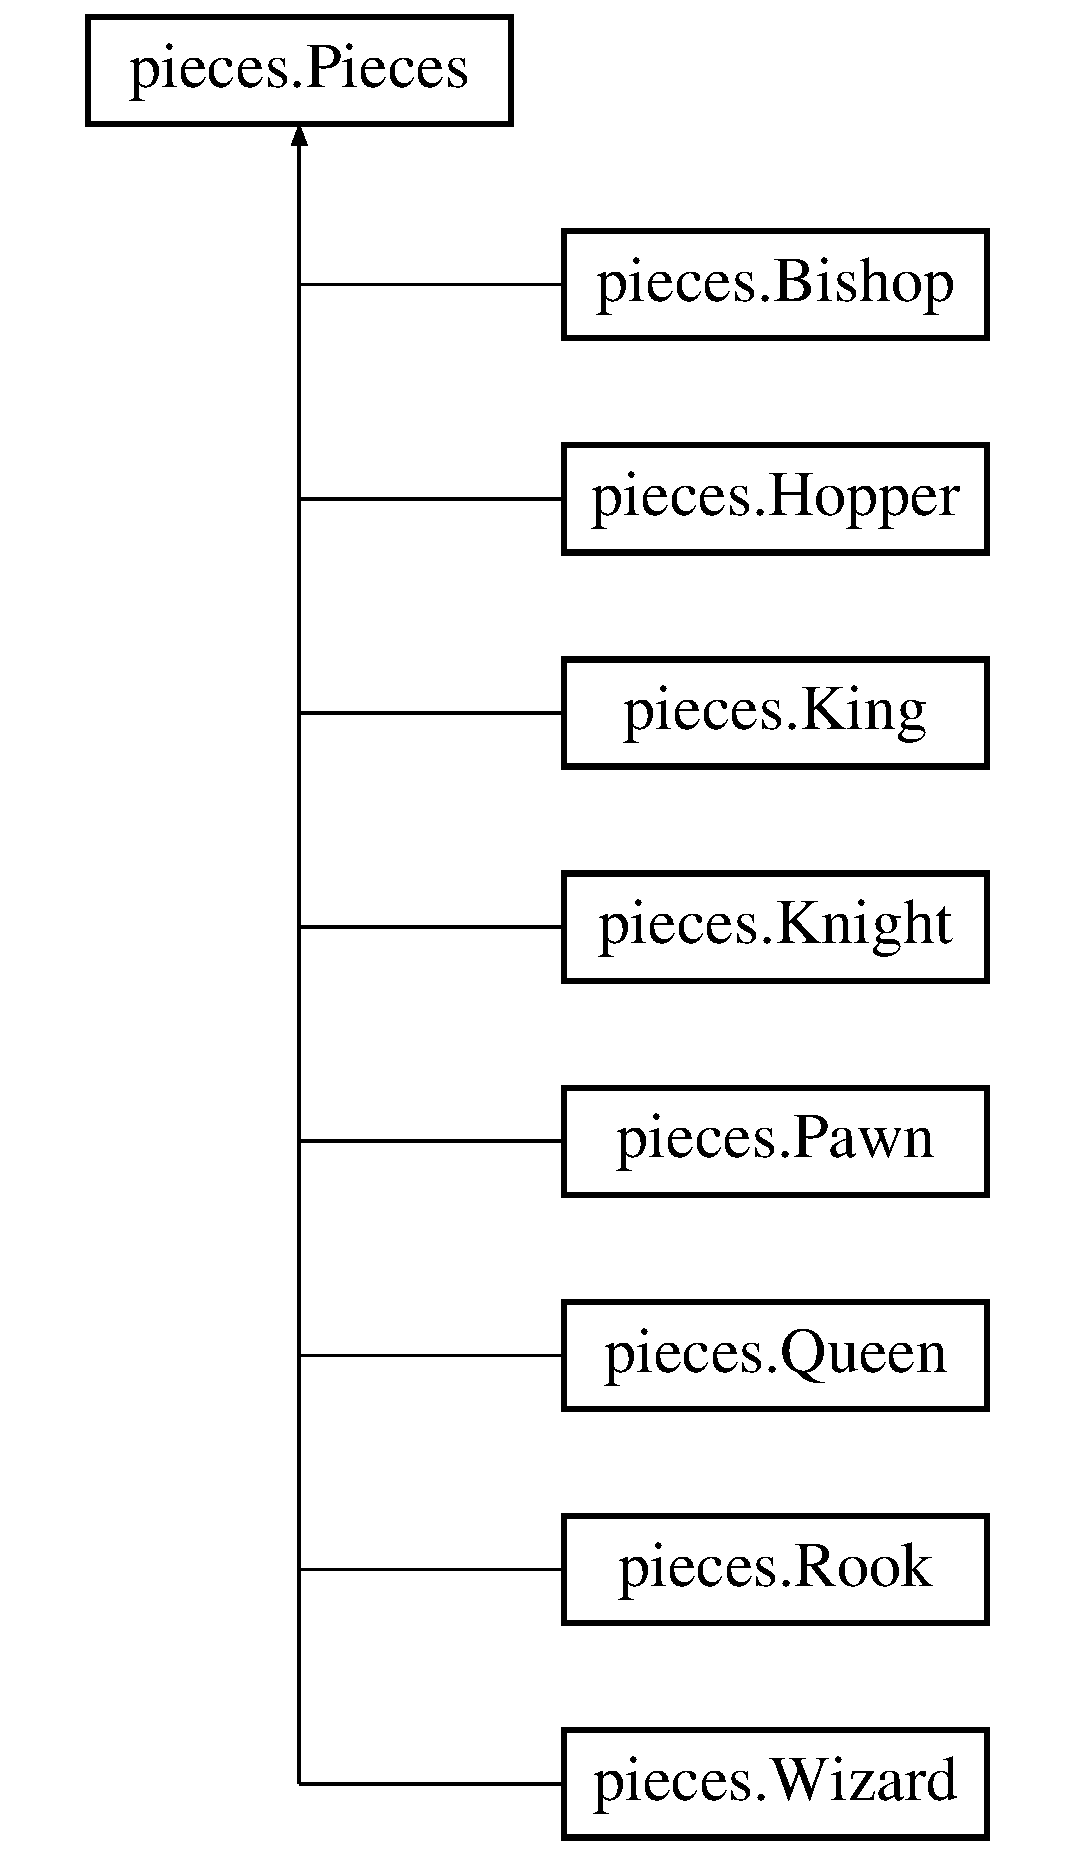
\includegraphics[height=9.000000cm]{classpieces_1_1_pieces}
\end{center}
\end{figure}
\subsection*{Public Member Functions}
\begin{DoxyCompactItemize}
\item 
\mbox{\Hypertarget{classpieces_1_1_pieces_a591cca84e6cf37ac52f1aff44d00764e}\label{classpieces_1_1_pieces_a591cca84e6cf37ac52f1aff44d00764e}} 
{\bfseries Pieces} (int \mbox{\hyperlink{classpieces_1_1_pieces_ac5178f9b8a6b0c4235851475081249f3}{x}}, int \mbox{\hyperlink{classpieces_1_1_pieces_a66d911734967a8ced1b9792fe900fadb}{y}}, \mbox{\hyperlink{classgame_1_1_player}{Player}} \mbox{\hyperlink{classpieces_1_1_pieces_a49f35044dd36e5c4b04261a8ea54ad0c}{player}})
\item 
\mbox{\Hypertarget{classpieces_1_1_pieces_aad794f16bdefb770c3bba9a8036929cf}\label{classpieces_1_1_pieces_aad794f16bdefb770c3bba9a8036929cf}} 
int \mbox{[}$\,$\mbox{]} {\bfseries get\+Position} ()
\item 
\mbox{\Hypertarget{classpieces_1_1_pieces_a18d54763d5b7f5dd2e42cd1883819fa4}\label{classpieces_1_1_pieces_a18d54763d5b7f5dd2e42cd1883819fa4}} 
\mbox{\hyperlink{enumpieces_1_1_type}{Type}} {\bfseries get\+Type} ()
\item 
\mbox{\Hypertarget{classpieces_1_1_pieces_a077a98722aa3641b983f7c74c1377739}\label{classpieces_1_1_pieces_a077a98722aa3641b983f7c74c1377739}} 
\mbox{\hyperlink{classgame_1_1_player}{Player}} {\bfseries get\+Player} ()
\item 
abstract boolean \mbox{\hyperlink{classpieces_1_1_pieces_a4bdbd9bc2aa556e230e71a0cf756228f}{is\+Valid\+Move}} (int newX, int newY)
\item 
abstract List$<$ int\mbox{[}$\,$\mbox{]}$>$ \mbox{\hyperlink{classpieces_1_1_pieces_a28711472a94edf18be7c8300cf0cc64b}{moving}} (int newX, int newY)
\item 
void \mbox{\hyperlink{classpieces_1_1_pieces_aa204ec32ed62d79896561f253caf663a}{move}} (int newX, int newY)
\item 
void \mbox{\hyperlink{classpieces_1_1_pieces_ab54853b850ad823a067bdab91b907b86}{setX}} (int \mbox{\hyperlink{classpieces_1_1_pieces_ac5178f9b8a6b0c4235851475081249f3}{x}})
\item 
void \mbox{\hyperlink{classpieces_1_1_pieces_aefa2d9a29060faacd79e4e58d2c63196}{setY}} (int \mbox{\hyperlink{classpieces_1_1_pieces_a66d911734967a8ced1b9792fe900fadb}{y}})
\end{DoxyCompactItemize}
\subsection*{Public Attributes}
\begin{DoxyCompactItemize}
\item 
\mbox{\hyperlink{classgame_1_1_player}{Player}} \mbox{\hyperlink{classpieces_1_1_pieces_a49f35044dd36e5c4b04261a8ea54ad0c}{player}}
\item 
\mbox{\hyperlink{enumpieces_1_1_type}{Type}} \mbox{\hyperlink{classpieces_1_1_pieces_a74572cdf2d798e339c56827050259767}{type}}
\end{DoxyCompactItemize}
\subsection*{Protected Attributes}
\begin{DoxyCompactItemize}
\item 
int \mbox{\hyperlink{classpieces_1_1_pieces_ac5178f9b8a6b0c4235851475081249f3}{x}}
\item 
int \mbox{\hyperlink{classpieces_1_1_pieces_a66d911734967a8ced1b9792fe900fadb}{y}}
\end{DoxyCompactItemize}


\subsection{Member Function Documentation}
\mbox{\Hypertarget{classpieces_1_1_pieces_a4bdbd9bc2aa556e230e71a0cf756228f}\label{classpieces_1_1_pieces_a4bdbd9bc2aa556e230e71a0cf756228f}} 
\index{pieces\+::\+Pieces@{pieces\+::\+Pieces}!is\+Valid\+Move@{is\+Valid\+Move}}
\index{is\+Valid\+Move@{is\+Valid\+Move}!pieces\+::\+Pieces@{pieces\+::\+Pieces}}
\subsubsection{\texorpdfstring{is\+Valid\+Move()}{isValidMove()}}
{\footnotesize\ttfamily abstract boolean pieces.\+Pieces.\+is\+Valid\+Move (\begin{DoxyParamCaption}\item[{int}]{newX,  }\item[{int}]{newY }\end{DoxyParamCaption})\hspace{0.3cm}{\ttfamily [abstract]}}

check pieces follow their own rules 
\begin{DoxyParams}{Parameters}
{\em newX} & destination rank of the piece \\
\hline
{\em newY} & destination file of the piece \\
\hline
\end{DoxyParams}
\begin{DoxyReturn}{Returns}
whether this step is a valid move 
\end{DoxyReturn}
\mbox{\Hypertarget{classpieces_1_1_pieces_aa204ec32ed62d79896561f253caf663a}\label{classpieces_1_1_pieces_aa204ec32ed62d79896561f253caf663a}} 
\index{pieces\+::\+Pieces@{pieces\+::\+Pieces}!move@{move}}
\index{move@{move}!pieces\+::\+Pieces@{pieces\+::\+Pieces}}
\subsubsection{\texorpdfstring{move()}{move()}}
{\footnotesize\ttfamily void pieces.\+Pieces.\+move (\begin{DoxyParamCaption}\item[{int}]{newX,  }\item[{int}]{newY }\end{DoxyParamCaption})\hspace{0.3cm}{\ttfamily [inline]}}

update the piece position 
\begin{DoxyParams}{Parameters}
{\em newX} & destination rank of the piece \\
\hline
{\em newY} & destination file of the piece \\
\hline
\end{DoxyParams}
\mbox{\Hypertarget{classpieces_1_1_pieces_a28711472a94edf18be7c8300cf0cc64b}\label{classpieces_1_1_pieces_a28711472a94edf18be7c8300cf0cc64b}} 
\index{pieces\+::\+Pieces@{pieces\+::\+Pieces}!moving@{moving}}
\index{moving@{moving}!pieces\+::\+Pieces@{pieces\+::\+Pieces}}
\subsubsection{\texorpdfstring{moving()}{moving()}}
{\footnotesize\ttfamily abstract List$<$int\mbox{[}$\,$\mbox{]}$>$ pieces.\+Pieces.\+moving (\begin{DoxyParamCaption}\item[{int}]{newX,  }\item[{int}]{newY }\end{DoxyParamCaption})\hspace{0.3cm}{\ttfamily [abstract]}}

store the passing positions a helper function for later check leap over other pieces 
\begin{DoxyParams}{Parameters}
{\em newX} & destination rank of the piece \\
\hline
{\em newY} & destination file of the piece \\
\hline
\end{DoxyParams}
\begin{DoxyReturn}{Returns}
a list of squares that the piece passing 
\end{DoxyReturn}
\mbox{\Hypertarget{classpieces_1_1_pieces_ab54853b850ad823a067bdab91b907b86}\label{classpieces_1_1_pieces_ab54853b850ad823a067bdab91b907b86}} 
\index{pieces\+::\+Pieces@{pieces\+::\+Pieces}!setX@{setX}}
\index{setX@{setX}!pieces\+::\+Pieces@{pieces\+::\+Pieces}}
\subsubsection{\texorpdfstring{set\+X()}{setX()}}
{\footnotesize\ttfamily void pieces.\+Pieces.\+setX (\begin{DoxyParamCaption}\item[{int}]{x }\end{DoxyParamCaption})\hspace{0.3cm}{\ttfamily [inline]}}

set piece\textquotesingle{}s rank position 
\begin{DoxyParams}{Parameters}
{\em x} & new rank position \\
\hline
\end{DoxyParams}
\mbox{\Hypertarget{classpieces_1_1_pieces_aefa2d9a29060faacd79e4e58d2c63196}\label{classpieces_1_1_pieces_aefa2d9a29060faacd79e4e58d2c63196}} 
\index{pieces\+::\+Pieces@{pieces\+::\+Pieces}!setY@{setY}}
\index{setY@{setY}!pieces\+::\+Pieces@{pieces\+::\+Pieces}}
\subsubsection{\texorpdfstring{set\+Y()}{setY()}}
{\footnotesize\ttfamily void pieces.\+Pieces.\+setY (\begin{DoxyParamCaption}\item[{int}]{y }\end{DoxyParamCaption})\hspace{0.3cm}{\ttfamily [inline]}}

set piece\textquotesingle{}s file position 
\begin{DoxyParams}{Parameters}
{\em y} & new file position \\
\hline
\end{DoxyParams}


\subsection{Member Data Documentation}
\mbox{\Hypertarget{classpieces_1_1_pieces_a49f35044dd36e5c4b04261a8ea54ad0c}\label{classpieces_1_1_pieces_a49f35044dd36e5c4b04261a8ea54ad0c}} 
\index{pieces\+::\+Pieces@{pieces\+::\+Pieces}!player@{player}}
\index{player@{player}!pieces\+::\+Pieces@{pieces\+::\+Pieces}}
\subsubsection{\texorpdfstring{player}{player}}
{\footnotesize\ttfamily \mbox{\hyperlink{classgame_1_1_player}{Player}} pieces.\+Pieces.\+player}

the player piece belongs to \mbox{\Hypertarget{classpieces_1_1_pieces_a74572cdf2d798e339c56827050259767}\label{classpieces_1_1_pieces_a74572cdf2d798e339c56827050259767}} 
\index{pieces\+::\+Pieces@{pieces\+::\+Pieces}!type@{type}}
\index{type@{type}!pieces\+::\+Pieces@{pieces\+::\+Pieces}}
\subsubsection{\texorpdfstring{type}{type}}
{\footnotesize\ttfamily \mbox{\hyperlink{enumpieces_1_1_type}{Type}} pieces.\+Pieces.\+type}

the type the piece should be \mbox{\Hypertarget{classpieces_1_1_pieces_ac5178f9b8a6b0c4235851475081249f3}\label{classpieces_1_1_pieces_ac5178f9b8a6b0c4235851475081249f3}} 
\index{pieces\+::\+Pieces@{pieces\+::\+Pieces}!x@{x}}
\index{x@{x}!pieces\+::\+Pieces@{pieces\+::\+Pieces}}
\subsubsection{\texorpdfstring{x}{x}}
{\footnotesize\ttfamily int pieces.\+Pieces.\+x\hspace{0.3cm}{\ttfamily [protected]}}

rank position of the piece \mbox{\Hypertarget{classpieces_1_1_pieces_a66d911734967a8ced1b9792fe900fadb}\label{classpieces_1_1_pieces_a66d911734967a8ced1b9792fe900fadb}} 
\index{pieces\+::\+Pieces@{pieces\+::\+Pieces}!y@{y}}
\index{y@{y}!pieces\+::\+Pieces@{pieces\+::\+Pieces}}
\subsubsection{\texorpdfstring{y}{y}}
{\footnotesize\ttfamily int pieces.\+Pieces.\+y\hspace{0.3cm}{\ttfamily [protected]}}

file position of the piece 

The documentation for this class was generated from the following file\+:\begin{DoxyCompactItemize}
\item 
src/pieces/Pieces.\+java\end{DoxyCompactItemize}

\hypertarget{classgame_1_1_player}{}\section{game.\+Player Class Reference}
\label{classgame_1_1_player}\index{game.\+Player@{game.\+Player}}
\subsection*{Public Member Functions}
\begin{DoxyCompactItemize}
\item 
\mbox{\hyperlink{classgame_1_1_player_ab50e8fdec094890642f652d2529356e7}{Player}} (int \mbox{\hyperlink{classgame_1_1_player_a78e50f5f23d0c3f75abb86e1e9c6f63d}{color}}, \mbox{\hyperlink{classgame_1_1_board}{Board}} \mbox{\hyperlink{classgame_1_1_player_a00d2553d16a3ade53d5671421fa8dcf6}{play\+Board}})
\item 
void \mbox{\hyperlink{classgame_1_1_player_a936532b865afe0eb13cf4bbc490c78f8}{get\+Pieces}} (List$<$ \mbox{\hyperlink{classpieces_1_1_pieces}{Pieces}} $>$ \mbox{\hyperlink{classgame_1_1_player_a9028dcf4027ecd82c1d9494f7e304960}{pieces}})
\item 
boolean \mbox{\hyperlink{classgame_1_1_player_a7d2facf4888849be1ffcab77f12eccd5}{has\+The\+Piece}} (\mbox{\hyperlink{classpieces_1_1_pieces}{Pieces}} p)
\end{DoxyCompactItemize}
\subsection*{Public Attributes}
\begin{DoxyCompactItemize}
\item 
int \mbox{\hyperlink{classgame_1_1_player_a78e50f5f23d0c3f75abb86e1e9c6f63d}{color}}
\item 
List$<$ \mbox{\hyperlink{classpieces_1_1_pieces}{Pieces}} $>$ \mbox{\hyperlink{classgame_1_1_player_a9028dcf4027ecd82c1d9494f7e304960}{pieces}}
\item 
boolean \mbox{\hyperlink{classgame_1_1_player_a55490a38f00ba09f4d6fab5ea6d57de7}{is\+Checked}}
\item 
\mbox{\hyperlink{classgame_1_1_board}{Board}} \mbox{\hyperlink{classgame_1_1_player_a00d2553d16a3ade53d5671421fa8dcf6}{play\+Board}}
\item 
boolean \mbox{\hyperlink{classgame_1_1_player_a3016e4b3cc8dae43ad3e08d31c8a5e3b}{is\+Lose}}
\end{DoxyCompactItemize}


\subsection{Detailed Description}
\mbox{\hyperlink{classgame_1_1_player}{Player}} class which contains player information. 

\subsection{Constructor \& Destructor Documentation}
\mbox{\Hypertarget{classgame_1_1_player_ab50e8fdec094890642f652d2529356e7}\label{classgame_1_1_player_ab50e8fdec094890642f652d2529356e7}} 
\index{game\+::\+Player@{game\+::\+Player}!Player@{Player}}
\index{Player@{Player}!game\+::\+Player@{game\+::\+Player}}
\subsubsection{\texorpdfstring{Player()}{Player()}}
{\footnotesize\ttfamily game.\+Player.\+Player (\begin{DoxyParamCaption}\item[{int}]{color,  }\item[{\mbox{\hyperlink{classgame_1_1_board}{Board}}}]{play\+Board }\end{DoxyParamCaption})\hspace{0.3cm}{\ttfamily [inline]}}

initialize player attributes 
\begin{DoxyParams}{Parameters}
{\em color} & the color of player\textquotesingle{}s pieces \\
\hline
{\em play\+Board} & the board that player is playing on \\
\hline
\end{DoxyParams}


\subsection{Member Function Documentation}
\mbox{\Hypertarget{classgame_1_1_player_a936532b865afe0eb13cf4bbc490c78f8}\label{classgame_1_1_player_a936532b865afe0eb13cf4bbc490c78f8}} 
\index{game\+::\+Player@{game\+::\+Player}!get\+Pieces@{get\+Pieces}}
\index{get\+Pieces@{get\+Pieces}!game\+::\+Player@{game\+::\+Player}}
\subsubsection{\texorpdfstring{get\+Pieces()}{getPieces()}}
{\footnotesize\ttfamily void game.\+Player.\+get\+Pieces (\begin{DoxyParamCaption}\item[{List$<$ \mbox{\hyperlink{classpieces_1_1_pieces}{Pieces}} $>$}]{pieces }\end{DoxyParamCaption})\hspace{0.3cm}{\ttfamily [inline]}}

assign pieces on the board to the player 
\begin{DoxyParams}{Parameters}
{\em pieces} & a list of pieces given to the player \\
\hline
\end{DoxyParams}
\mbox{\Hypertarget{classgame_1_1_player_a7d2facf4888849be1ffcab77f12eccd5}\label{classgame_1_1_player_a7d2facf4888849be1ffcab77f12eccd5}} 
\index{game\+::\+Player@{game\+::\+Player}!has\+The\+Piece@{has\+The\+Piece}}
\index{has\+The\+Piece@{has\+The\+Piece}!game\+::\+Player@{game\+::\+Player}}
\subsubsection{\texorpdfstring{has\+The\+Piece()}{hasThePiece()}}
{\footnotesize\ttfamily boolean game.\+Player.\+has\+The\+Piece (\begin{DoxyParamCaption}\item[{\mbox{\hyperlink{classpieces_1_1_pieces}{Pieces}}}]{p }\end{DoxyParamCaption})\hspace{0.3cm}{\ttfamily [inline]}}

check whether this player has this piece 
\begin{DoxyParams}{Parameters}
{\em p} & the piece being checked \\
\hline
\end{DoxyParams}
\begin{DoxyReturn}{Returns}
whether the piece exists in player\textquotesingle{}s pieces list 
\end{DoxyReturn}


\subsection{Member Data Documentation}
\mbox{\Hypertarget{classgame_1_1_player_a78e50f5f23d0c3f75abb86e1e9c6f63d}\label{classgame_1_1_player_a78e50f5f23d0c3f75abb86e1e9c6f63d}} 
\index{game\+::\+Player@{game\+::\+Player}!color@{color}}
\index{color@{color}!game\+::\+Player@{game\+::\+Player}}
\subsubsection{\texorpdfstring{color}{color}}
{\footnotesize\ttfamily int game.\+Player.\+color}

the color of pieces \mbox{\Hypertarget{classgame_1_1_player_a55490a38f00ba09f4d6fab5ea6d57de7}\label{classgame_1_1_player_a55490a38f00ba09f4d6fab5ea6d57de7}} 
\index{game\+::\+Player@{game\+::\+Player}!is\+Checked@{is\+Checked}}
\index{is\+Checked@{is\+Checked}!game\+::\+Player@{game\+::\+Player}}
\subsubsection{\texorpdfstring{is\+Checked}{isChecked}}
{\footnotesize\ttfamily boolean game.\+Player.\+is\+Checked}

whether the player is in check \mbox{\Hypertarget{classgame_1_1_player_a3016e4b3cc8dae43ad3e08d31c8a5e3b}\label{classgame_1_1_player_a3016e4b3cc8dae43ad3e08d31c8a5e3b}} 
\index{game\+::\+Player@{game\+::\+Player}!is\+Lose@{is\+Lose}}
\index{is\+Lose@{is\+Lose}!game\+::\+Player@{game\+::\+Player}}
\subsubsection{\texorpdfstring{is\+Lose}{isLose}}
{\footnotesize\ttfamily boolean game.\+Player.\+is\+Lose}

whether the player is lose \mbox{\Hypertarget{classgame_1_1_player_a9028dcf4027ecd82c1d9494f7e304960}\label{classgame_1_1_player_a9028dcf4027ecd82c1d9494f7e304960}} 
\index{game\+::\+Player@{game\+::\+Player}!pieces@{pieces}}
\index{pieces@{pieces}!game\+::\+Player@{game\+::\+Player}}
\subsubsection{\texorpdfstring{pieces}{pieces}}
{\footnotesize\ttfamily List$<$\mbox{\hyperlink{classpieces_1_1_pieces}{Pieces}}$>$ game.\+Player.\+pieces}

a list of pieces the player owned \mbox{\Hypertarget{classgame_1_1_player_a00d2553d16a3ade53d5671421fa8dcf6}\label{classgame_1_1_player_a00d2553d16a3ade53d5671421fa8dcf6}} 
\index{game\+::\+Player@{game\+::\+Player}!play\+Board@{play\+Board}}
\index{play\+Board@{play\+Board}!game\+::\+Player@{game\+::\+Player}}
\subsubsection{\texorpdfstring{play\+Board}{playBoard}}
{\footnotesize\ttfamily \mbox{\hyperlink{classgame_1_1_board}{Board}} game.\+Player.\+play\+Board}

board the player is playing on 

The documentation for this class was generated from the following file\+:\begin{DoxyCompactItemize}
\item 
src/game/Player.\+java\end{DoxyCompactItemize}

\hypertarget{classpieces_1_1_queen}{}\section{pieces.\+Queen Class Reference}
\label{classpieces_1_1_queen}\index{pieces.\+Queen@{pieces.\+Queen}}
Inheritance diagram for pieces.\+Queen\+:\begin{figure}[H]
\begin{center}
\leavevmode
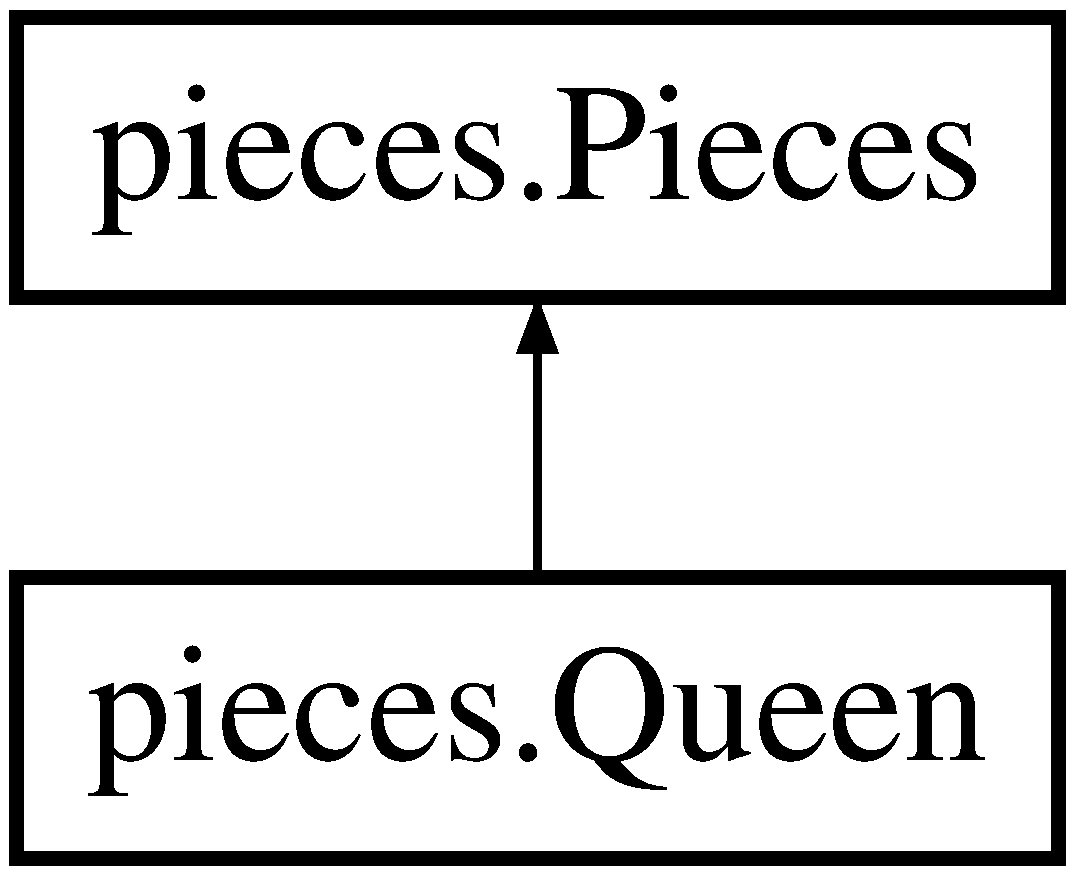
\includegraphics[height=2.000000cm]{classpieces_1_1_queen}
\end{center}
\end{figure}
\subsection*{Public Member Functions}
\begin{DoxyCompactItemize}
\item 
\mbox{\hyperlink{classpieces_1_1_queen_a330bbe8bd6a75147004ed3267b0b422f}{Queen}} (int \mbox{\hyperlink{classpieces_1_1_pieces_ac5178f9b8a6b0c4235851475081249f3}{x}}, int \mbox{\hyperlink{classpieces_1_1_pieces_a66d911734967a8ced1b9792fe900fadb}{y}}, \mbox{\hyperlink{classgame_1_1_player}{Player}} \mbox{\hyperlink{classpieces_1_1_pieces_a49f35044dd36e5c4b04261a8ea54ad0c}{player}})
\item 
boolean \mbox{\hyperlink{classpieces_1_1_queen_a12c3d1bc54998da5947802f70070378f}{is\+Valid\+Move}} (int newX, int newY)
\item 
List$<$ int\mbox{[}$\,$\mbox{]}$>$ \mbox{\hyperlink{classpieces_1_1_queen_a2e0d378c18cf3fd85dc1acf860294950}{moving}} (int newX, int newY)
\end{DoxyCompactItemize}
\subsection*{Additional Inherited Members}


\subsection{Detailed Description}
\mbox{\hyperlink{classpieces_1_1_queen}{Queen}} class 

The queen combines the power of the rook and bishop and can move any number of squares along rank, file, or diagonal, but it may not leap over other pieces. 

\subsection{Constructor \& Destructor Documentation}
\mbox{\Hypertarget{classpieces_1_1_queen_a330bbe8bd6a75147004ed3267b0b422f}\label{classpieces_1_1_queen_a330bbe8bd6a75147004ed3267b0b422f}} 
\index{pieces\+::\+Queen@{pieces\+::\+Queen}!Queen@{Queen}}
\index{Queen@{Queen}!pieces\+::\+Queen@{pieces\+::\+Queen}}
\subsubsection{\texorpdfstring{Queen()}{Queen()}}
{\footnotesize\ttfamily pieces.\+Queen.\+Queen (\begin{DoxyParamCaption}\item[{int}]{x,  }\item[{int}]{y,  }\item[{\mbox{\hyperlink{classgame_1_1_player}{Player}}}]{player }\end{DoxyParamCaption})\hspace{0.3cm}{\ttfamily [inline]}}

initialize queen attributes 
\begin{DoxyParams}{Parameters}
{\em x} & the initial rank position \\
\hline
{\em y} & the initial file position \\
\hline
{\em player} & the player piece belong to \\
\hline
\end{DoxyParams}


\subsection{Member Function Documentation}
\mbox{\Hypertarget{classpieces_1_1_queen_a12c3d1bc54998da5947802f70070378f}\label{classpieces_1_1_queen_a12c3d1bc54998da5947802f70070378f}} 
\index{pieces\+::\+Queen@{pieces\+::\+Queen}!is\+Valid\+Move@{is\+Valid\+Move}}
\index{is\+Valid\+Move@{is\+Valid\+Move}!pieces\+::\+Queen@{pieces\+::\+Queen}}
\subsubsection{\texorpdfstring{is\+Valid\+Move()}{isValidMove()}}
{\footnotesize\ttfamily boolean pieces.\+Queen.\+is\+Valid\+Move (\begin{DoxyParamCaption}\item[{int}]{newX,  }\item[{int}]{newY }\end{DoxyParamCaption})\hspace{0.3cm}{\ttfamily [inline]}}

check whether queen is moved by its own rule; queen could move in all eight directions 
\begin{DoxyParams}{Parameters}
{\em newX} & destination rank of the piece \\
\hline
{\em newY} & destination file of the piece \\
\hline
\end{DoxyParams}
\begin{DoxyReturn}{Returns}
whether this step is a valid move 
\end{DoxyReturn}
\mbox{\Hypertarget{classpieces_1_1_queen_a2e0d378c18cf3fd85dc1acf860294950}\label{classpieces_1_1_queen_a2e0d378c18cf3fd85dc1acf860294950}} 
\index{pieces\+::\+Queen@{pieces\+::\+Queen}!moving@{moving}}
\index{moving@{moving}!pieces\+::\+Queen@{pieces\+::\+Queen}}
\subsubsection{\texorpdfstring{moving()}{moving()}}
{\footnotesize\ttfamily List$<$int\mbox{[}$\,$\mbox{]}$>$ pieces.\+Queen.\+moving (\begin{DoxyParamCaption}\item[{int}]{newX,  }\item[{int}]{newY }\end{DoxyParamCaption})\hspace{0.3cm}{\ttfamily [inline]}}

store the passing positions a helper function for later check leap over other pieces since \mbox{\hyperlink{classpieces_1_1_queen}{Queen}} combines rules of \mbox{\hyperlink{classpieces_1_1_rook}{Rook}} and \mbox{\hyperlink{classpieces_1_1_bishop}{Bishop}}, apply methods in both classes 
\begin{DoxyParams}{Parameters}
{\em newX} & destination rank of the piece \\
\hline
{\em newY} & destination file of the piece \\
\hline
\end{DoxyParams}
\begin{DoxyReturn}{Returns}
the positions that queen has leaped over 
\end{DoxyReturn}


The documentation for this class was generated from the following file\+:\begin{DoxyCompactItemize}
\item 
src/pieces/Queen.\+java\end{DoxyCompactItemize}

\hypertarget{classpieces_1_1_rook}{}\section{pieces.\+Rook Class Reference}
\label{classpieces_1_1_rook}\index{pieces.\+Rook@{pieces.\+Rook}}
Inheritance diagram for pieces.\+Rook\+:\begin{figure}[H]
\begin{center}
\leavevmode
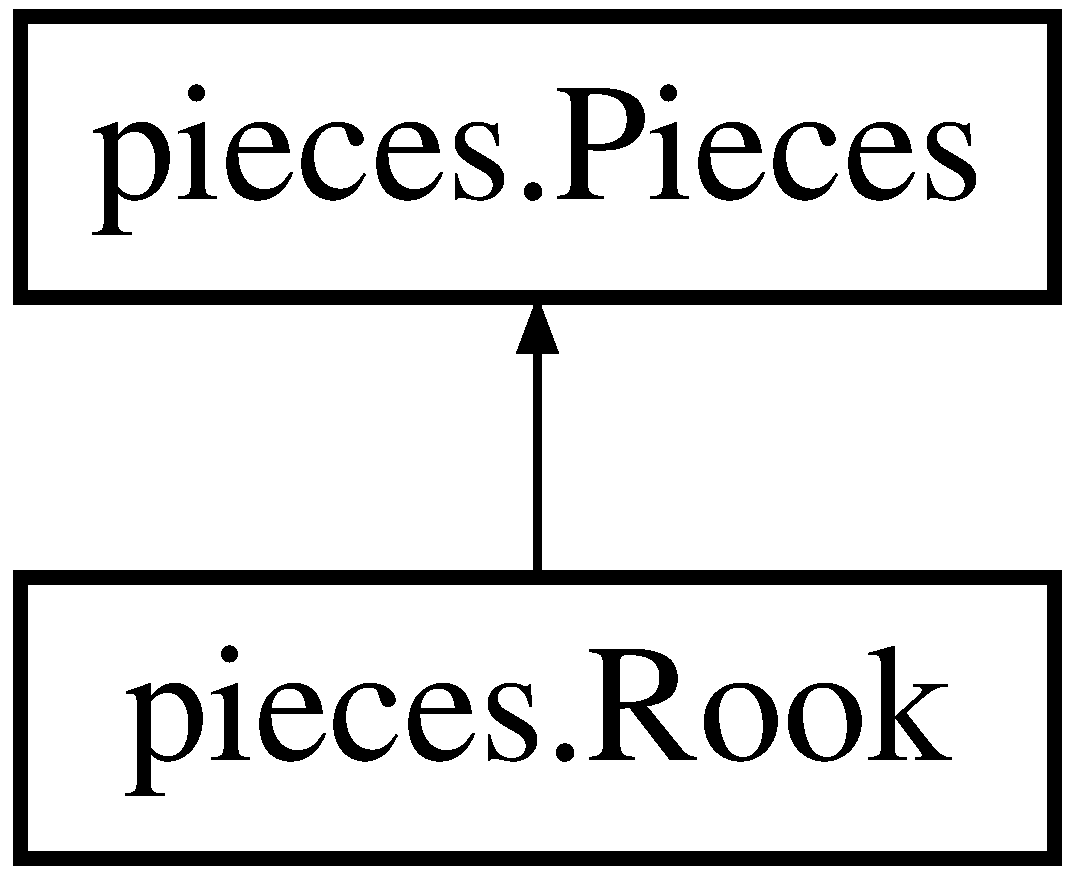
\includegraphics[height=2.000000cm]{classpieces_1_1_rook}
\end{center}
\end{figure}
\subsection*{Public Member Functions}
\begin{DoxyCompactItemize}
\item 
\mbox{\hyperlink{classpieces_1_1_rook_a9d77f8808929d292302628ad144b38a7}{Rook}} (int \mbox{\hyperlink{classpieces_1_1_pieces_ac5178f9b8a6b0c4235851475081249f3}{x}}, int \mbox{\hyperlink{classpieces_1_1_pieces_a66d911734967a8ced1b9792fe900fadb}{y}}, \mbox{\hyperlink{classgame_1_1_player}{Player}} \mbox{\hyperlink{classpieces_1_1_pieces_a49f35044dd36e5c4b04261a8ea54ad0c}{player}})
\item 
boolean \mbox{\hyperlink{classpieces_1_1_rook_a7c4ba4f45c9884e16b68e66521bbefb5}{is\+Valid\+Move}} (int newX, int newY)
\item 
List$<$ int\mbox{[}$\,$\mbox{]}$>$ \mbox{\hyperlink{classpieces_1_1_rook_a45ac73bc8b0a1b8efac9ec3b6398bb2c}{moving}} (int newX, int newY)
\end{DoxyCompactItemize}
\subsection*{Additional Inherited Members}


\subsection{Detailed Description}
\mbox{\hyperlink{classpieces_1_1_rook}{Rook}} Class 

The rook can move any number of squares along any rank or file, but may not leap over other pieces. 

\subsection{Constructor \& Destructor Documentation}
\mbox{\Hypertarget{classpieces_1_1_rook_a9d77f8808929d292302628ad144b38a7}\label{classpieces_1_1_rook_a9d77f8808929d292302628ad144b38a7}} 
\index{pieces\+::\+Rook@{pieces\+::\+Rook}!Rook@{Rook}}
\index{Rook@{Rook}!pieces\+::\+Rook@{pieces\+::\+Rook}}
\subsubsection{\texorpdfstring{Rook()}{Rook()}}
{\footnotesize\ttfamily pieces.\+Rook.\+Rook (\begin{DoxyParamCaption}\item[{int}]{x,  }\item[{int}]{y,  }\item[{\mbox{\hyperlink{classgame_1_1_player}{Player}}}]{player }\end{DoxyParamCaption})\hspace{0.3cm}{\ttfamily [inline]}}

initialize queen attributes 
\begin{DoxyParams}{Parameters}
{\em x} & the initial rank position \\
\hline
{\em y} & the initial file position \\
\hline
{\em player} & the player piece belong to \\
\hline
\end{DoxyParams}


\subsection{Member Function Documentation}
\mbox{\Hypertarget{classpieces_1_1_rook_a7c4ba4f45c9884e16b68e66521bbefb5}\label{classpieces_1_1_rook_a7c4ba4f45c9884e16b68e66521bbefb5}} 
\index{pieces\+::\+Rook@{pieces\+::\+Rook}!is\+Valid\+Move@{is\+Valid\+Move}}
\index{is\+Valid\+Move@{is\+Valid\+Move}!pieces\+::\+Rook@{pieces\+::\+Rook}}
\subsubsection{\texorpdfstring{is\+Valid\+Move()}{isValidMove()}}
{\footnotesize\ttfamily boolean pieces.\+Rook.\+is\+Valid\+Move (\begin{DoxyParamCaption}\item[{int}]{newX,  }\item[{int}]{newY }\end{DoxyParamCaption})\hspace{0.3cm}{\ttfamily [inline]}}

check whether rook is moved by its own rule; rook could only move along file or rank \mbox{\Hypertarget{classpieces_1_1_rook_a45ac73bc8b0a1b8efac9ec3b6398bb2c}\label{classpieces_1_1_rook_a45ac73bc8b0a1b8efac9ec3b6398bb2c}} 
\index{pieces\+::\+Rook@{pieces\+::\+Rook}!moving@{moving}}
\index{moving@{moving}!pieces\+::\+Rook@{pieces\+::\+Rook}}
\subsubsection{\texorpdfstring{moving()}{moving()}}
{\footnotesize\ttfamily List$<$int\mbox{[}$\,$\mbox{]}$>$ pieces.\+Rook.\+moving (\begin{DoxyParamCaption}\item[{int}]{newX,  }\item[{int}]{newY }\end{DoxyParamCaption})\hspace{0.3cm}{\ttfamily [inline]}}


\begin{DoxyParams}{Parameters}
{\em newX} & \\
\hline
{\em newY} & \\
\hline
\end{DoxyParams}
\begin{DoxyReturn}{Returns}
store the positions that rook has been leaped over 
\end{DoxyReturn}


The documentation for this class was generated from the following file\+:\begin{DoxyCompactItemize}
\item 
src/pieces/Rook.\+java\end{DoxyCompactItemize}

\hypertarget{enumpieces_1_1_type}{}\section{pieces.\+Type Enum Reference}
\label{enumpieces_1_1_type}\index{pieces.\+Type@{pieces.\+Type}}
\subsection*{Public Attributes}
\begin{DoxyCompactItemize}
\item 
\mbox{\Hypertarget{enumpieces_1_1_type_a94a5469a53ed2dc383b045595747ac2e}\label{enumpieces_1_1_type_a94a5469a53ed2dc383b045595747ac2e}} 
{\bfseries King}
\item 
\mbox{\Hypertarget{enumpieces_1_1_type_a7254feb0d571c38a786fc77345c19e44}\label{enumpieces_1_1_type_a7254feb0d571c38a786fc77345c19e44}} 
{\bfseries Rook}
\item 
\mbox{\Hypertarget{enumpieces_1_1_type_ae0247f7ae0004f10a225be7c8d240ea8}\label{enumpieces_1_1_type_ae0247f7ae0004f10a225be7c8d240ea8}} 
{\bfseries Bishop}
\item 
\mbox{\Hypertarget{enumpieces_1_1_type_a2393ad0192515b79b7fb7139aee566b2}\label{enumpieces_1_1_type_a2393ad0192515b79b7fb7139aee566b2}} 
{\bfseries Queen}
\item 
\mbox{\Hypertarget{enumpieces_1_1_type_ab19c5ea436b93fd98e23c09fef7943f7}\label{enumpieces_1_1_type_ab19c5ea436b93fd98e23c09fef7943f7}} 
{\bfseries Knight}
\item 
\mbox{\Hypertarget{enumpieces_1_1_type_a23aa2fdce43266a04b08bccef0cc2ae9}\label{enumpieces_1_1_type_a23aa2fdce43266a04b08bccef0cc2ae9}} 
{\bfseries Pawn}
\item 
\mbox{\Hypertarget{enumpieces_1_1_type_aab9cddf0bc06828bf34b0858ea5f139c}\label{enumpieces_1_1_type_aab9cddf0bc06828bf34b0858ea5f139c}} 
{\bfseries Wizard}
\item 
\mbox{\Hypertarget{enumpieces_1_1_type_a999780ebdab2950a4ec39a9f1b8ac166}\label{enumpieces_1_1_type_a999780ebdab2950a4ec39a9f1b8ac166}} 
{\bfseries Hopper}
\end{DoxyCompactItemize}


The documentation for this enum was generated from the following file\+:\begin{DoxyCompactItemize}
\item 
src/pieces/Type.\+java\end{DoxyCompactItemize}

\hypertarget{classpieces_1_1_wizard}{}\section{pieces.\+Wizard Class Reference}
\label{classpieces_1_1_wizard}\index{pieces.\+Wizard@{pieces.\+Wizard}}
Inheritance diagram for pieces.\+Wizard\+:\begin{figure}[H]
\begin{center}
\leavevmode
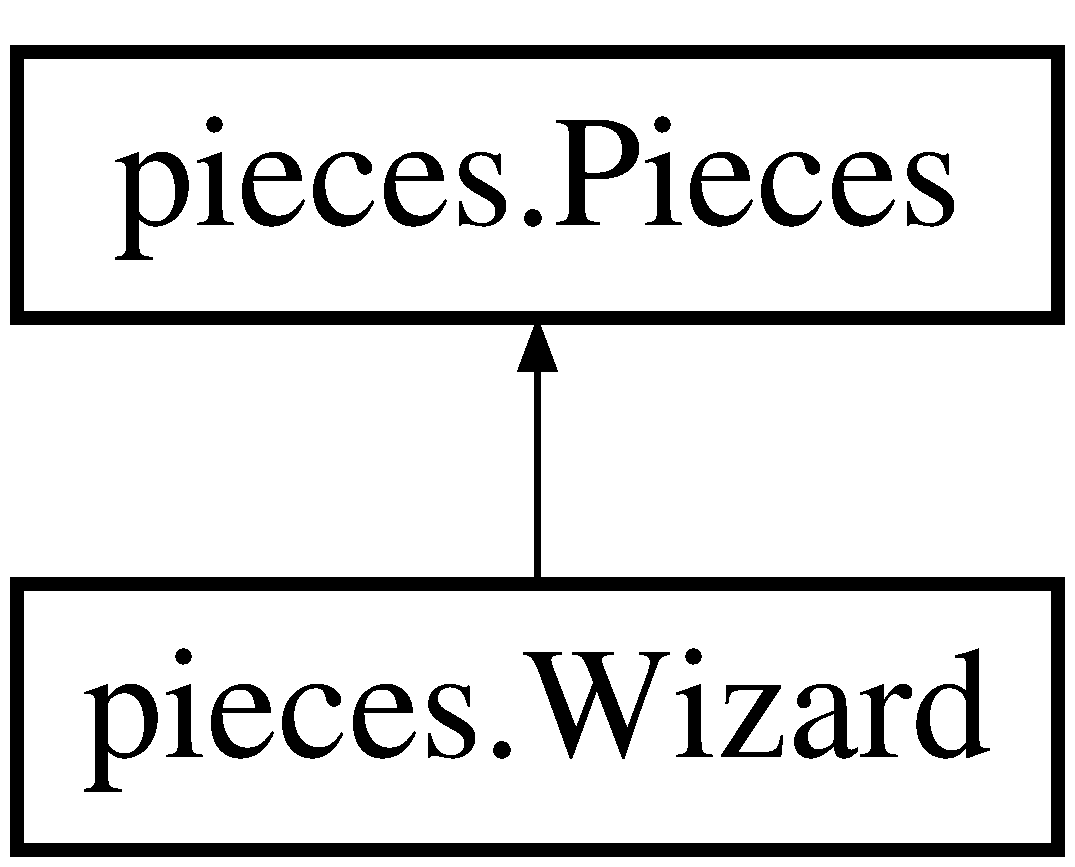
\includegraphics[height=2.000000cm]{classpieces_1_1_wizard}
\end{center}
\end{figure}
\subsection*{Public Member Functions}
\begin{DoxyCompactItemize}
\item 
\mbox{\hyperlink{classpieces_1_1_wizard_a33267d1b4e462ecc51b2a77d454ea98e}{Wizard}} (int \mbox{\hyperlink{classpieces_1_1_pieces_ac5178f9b8a6b0c4235851475081249f3}{x}}, int \mbox{\hyperlink{classpieces_1_1_pieces_a66d911734967a8ced1b9792fe900fadb}{y}}, \mbox{\hyperlink{classgame_1_1_player}{Player}} \mbox{\hyperlink{classpieces_1_1_pieces_a49f35044dd36e5c4b04261a8ea54ad0c}{player}})
\item 
boolean \mbox{\hyperlink{classpieces_1_1_wizard_ac8894909924ae970cb63b68d131bf2da}{is\+Valid\+Move}} (int newX, int newY)
\item 
List$<$ int\mbox{[}$\,$\mbox{]}$>$ \mbox{\hyperlink{classpieces_1_1_wizard_a477ebc0284c9c2a16513a7a7c9dc224e}{moving}} (int newX, int newY)
\end{DoxyCompactItemize}
\subsection*{Additional Inherited Members}


\subsection{Detailed Description}
\mbox{\hyperlink{classpieces_1_1_wizard}{Wizard}} Class 

\mbox{\hyperlink{classpieces_1_1_wizard}{Wizard}} could only move one step in any directions, like a king the opponent piece in \mbox{\hyperlink{classpieces_1_1_wizard}{Wizard}}\textquotesingle{}s left, right, up or down position will be removed. 

\subsection{Constructor \& Destructor Documentation}
\mbox{\Hypertarget{classpieces_1_1_wizard_a33267d1b4e462ecc51b2a77d454ea98e}\label{classpieces_1_1_wizard_a33267d1b4e462ecc51b2a77d454ea98e}} 
\index{pieces\+::\+Wizard@{pieces\+::\+Wizard}!Wizard@{Wizard}}
\index{Wizard@{Wizard}!pieces\+::\+Wizard@{pieces\+::\+Wizard}}
\subsubsection{\texorpdfstring{Wizard()}{Wizard()}}
{\footnotesize\ttfamily pieces.\+Wizard.\+Wizard (\begin{DoxyParamCaption}\item[{int}]{x,  }\item[{int}]{y,  }\item[{\mbox{\hyperlink{classgame_1_1_player}{Player}}}]{player }\end{DoxyParamCaption})\hspace{0.3cm}{\ttfamily [inline]}}

initialize wizard attributes 
\begin{DoxyParams}{Parameters}
{\em x} & the initial rank position \\
\hline
{\em y} & the initial file position \\
\hline
{\em player} & the player piece belong to \\
\hline
\end{DoxyParams}


\subsection{Member Function Documentation}
\mbox{\Hypertarget{classpieces_1_1_wizard_ac8894909924ae970cb63b68d131bf2da}\label{classpieces_1_1_wizard_ac8894909924ae970cb63b68d131bf2da}} 
\index{pieces\+::\+Wizard@{pieces\+::\+Wizard}!is\+Valid\+Move@{is\+Valid\+Move}}
\index{is\+Valid\+Move@{is\+Valid\+Move}!pieces\+::\+Wizard@{pieces\+::\+Wizard}}
\subsubsection{\texorpdfstring{is\+Valid\+Move()}{isValidMove()}}
{\footnotesize\ttfamily boolean pieces.\+Wizard.\+is\+Valid\+Move (\begin{DoxyParamCaption}\item[{int}]{newX,  }\item[{int}]{newY }\end{DoxyParamCaption})\hspace{0.3cm}{\ttfamily [inline]}}

check whether wizard is moved by its own rule; wizard move similar to king 
\begin{DoxyParams}{Parameters}
{\em newX} & destination rank of the piece \\
\hline
{\em newY} & destination file of the piece \\
\hline
\end{DoxyParams}
\begin{DoxyReturn}{Returns}
whether this step is a valid move 
\end{DoxyReturn}
\mbox{\Hypertarget{classpieces_1_1_wizard_a477ebc0284c9c2a16513a7a7c9dc224e}\label{classpieces_1_1_wizard_a477ebc0284c9c2a16513a7a7c9dc224e}} 
\index{pieces\+::\+Wizard@{pieces\+::\+Wizard}!moving@{moving}}
\index{moving@{moving}!pieces\+::\+Wizard@{pieces\+::\+Wizard}}
\subsubsection{\texorpdfstring{moving()}{moving()}}
{\footnotesize\ttfamily List$<$int\mbox{[}$\,$\mbox{]}$>$ pieces.\+Wizard.\+moving (\begin{DoxyParamCaption}\item[{int}]{newX,  }\item[{int}]{newY }\end{DoxyParamCaption})\hspace{0.3cm}{\ttfamily [inline]}}

store the passing positions a helper function for later check leap over other pieces 
\begin{DoxyParams}{Parameters}
{\em newX} & destination rank of the piece \\
\hline
{\em newY} & destination file of the piece \\
\hline
\end{DoxyParams}
\begin{DoxyReturn}{Returns}
null, since wizard only move one squares each time 
\end{DoxyReturn}


The documentation for this class was generated from the following file\+:\begin{DoxyCompactItemize}
\item 
src/pieces/Wizard.\+java\end{DoxyCompactItemize}

%--- End generated contents ---

% Index
\backmatter
\newpage
\phantomsection
\clearemptydoublepage
\addcontentsline{toc}{chapter}{Index}
\printindex

\end{document}
